%! Mode:: "TeX:UTF-8"
%! TEX program = xelatex
\PassOptionsToPackage{quiet}{xeCJK}
\documentclass[withoutpreface,bwprint]{cumcmthesis}
\usepackage{etoolbox}
\BeforeBeginEnvironment{tabular}{\zihao{-5}}
\usepackage[framemethod=TikZ]{mdframed}  % 框架宏包
\usepackage{url}  % 网页链接宏包
\usepackage{setspace}
\usepackage{graphicx}
%%%%%%%%%%%%%%%%%%%%%%%%%%%%%%%%%%%%%%%%%%%%%%%%%%%%%%%%
%下面是美赛搬过来的usepackage
\usepackage{pgfplots}
\pgfplotsset{compat=1.18}
%\usepackage{palatino}  % 帕拉提诺体字体宏包
%\usepackage{times}  % 正文使用Times New Roman风格字体
%\usepackage{newtxmath}
\usepackage{lipsum}  % 导入生成段落的宏包
\usepackage{indentfirst}
\usepackage{booktabs} % For professional-looking tables
\usepackage{xcolor}   % For cell coloring
\usepackage{colortbl} % Required for \rowcolor
\definecolor{LightGreen}{rgb}{0.9, 0.95, 0.9}
\definecolor{LightBlue}{RGB}{229, 238, 255}
\definecolor{LightPink}{RGB}{255, 229, 237}
\usepackage{fancyhdr}
\usepackage{enumitem} % 用于自定义列表格式
\usepackage{setspace}
\usepackage{booktabs}  % 三线表加粗
\usepackage{float}
\usepackage{eso-pic}  % 用于在页面添加背景
\usepackage{graphicx} % 图片支持
\usepackage{tikz}     % 用于绘制半透明覆盖层
\usepackage{subcaption}
\usepackage{caption}
%\usepackage{nccmath}
%\everymath{\displaystyle} %全文行内公式自动启用displaystyle
\setlist[itemize]{listparindent=2em}
\setlist[enumerate]{listparindent=2em}
\setlength\parindent{2em}
\usepackage[titles]{tocloft}
\usepackage{tabularx}
\usepackage[titles]{tocloft}
\setlength{\cftbeforesecskip}{8pt}   % 节前间距
\setlength{\cftbeforesubsecskip}{4pt} % 小节前间距

\makeatletter
\renewcommand{\@seccntformat}[1]{\csname the#1\endcsname\hspace{1em}}
\makeatother%这四行是调subsub的空格

% 设置中文字体加粗使用黑体
\setCJKfamilyfont{bfsong}[AutoFakeBold=2]{SimHei}
\renewcommand{\bfseries}{\CJKfamily{bfsong}}


\urlstyle{rm}
\setlength{\headheight}{13.6pt}
\lstset{
    basicstyle=\footnotesize\ttfamily, % 字体大小和类型
    numbers=left,               % 在左侧显示行号
    numberstyle=\tiny,          % 设置行号字体
    numbersep=5pt,              % 行号与代码间距
    showspaces=false,           % 不显示空格
    showstringspaces=false,     % 字符串中不显示空格
    showtabs=false,             % 不显示制表符
    tabsize=2,                  % 制表符大小
    breaklines=true,            % 自动换行
    breakatwhitespace=false,    % 只在空格处换行
    title=\lstname,             % 显示文件名
    escapeinside={\%*}{*)},     % LaTeX代码嵌入
    xleftmargin=10pt,           % 左边距
    xrightmargin=10pt,          % 右边距
    aboveskip=5pt,              % 上方间距
    belowskip=5pt,              % 下方间距
    lineskip=-1pt               % 减小行距（负值可以压缩行距）
}
\newcolumntype{C}{>{\centering\arraybackslash}X}
\newcolumntype{R}{>{\raggedleft\arraybackslash}X}
\newcolumntype{L}{>{\raggedright\arraybackslash}X}
\renewcommand{\abstractname}{摘\kern1em要}
\title{基于物理状态转移方程的过滤器寿命预测与维护策略}  % 论文标题
\tihao{}  % 题号
\baominghao{}  % 报名号
\schoolname{}  % 学校
\membera{}  % 队员a
\memberb{}  % 队员b
\memberc{}  % 队员c
\supervisor{}  % 指导老师
\yearinput{}
\monthinput{}
\dayinput{}

%%%%%%%%%%%%%%%%%%%%%%%%%%%%%%%%%%%%%%%%%%%%%%%%%%%%%%%%%%%%%
%% 正文
\begin{document}

\maketitle
\begin{abstract}

在工业生产当中，污水需要经过过滤器净化后排放。在此过程中，污水过滤器的透水率会发生变化，下降到一定数值就无法使用，因此工厂需要对设备进行维护。依据某工厂两年过滤器透水率的实时监测情况，本文主要研究回应透水率变化与过滤器寿命的规律、使得工厂污水净化年成本最小的过滤器维护方案。通过\textbf{STL时间序列分解}、\textbf{物理状态转移方程}、\textbf{遗传算法}等进行求解。

\textbf{针对问题一}：采用\textbf{改进的自适应Hampel滤波器}进行数据清洗，通过\textbf{两阶段检测策略}有效剔除了异常值并保留了维护引发的真实阶跃信号，使用线性插值填补缺失值减小数据偏差。
通过\textbf{STL时间序列分解}得出透水率以一年为周期的波动特征，采用\textbf{快速傅里叶变换}与\textbf{自相关系数}验证结论。利用季节影响算子、劣化斜率得出透水率夏季劣化慢、秋冬季劣化快，且劣化速度随使用年限加快的下降规律。
引入维护增益与维护损伤系数，量化不同维护类型的瞬时恢复效果和长期损伤累积。
最后提取了刻画透水率变化的四项核心指标：\textbf{基准劣化率}反映无维护干预下过滤器的自然衰减速度；\textbf{季节影响算子}量化季节因素对透水率的影响；\textbf{维护增益}描述不同维护操作对透水率的瞬时提升效果；\textbf{维护损伤系数}则衡量维护活动对过滤器长期劣化速率的加速效应。

\textbf{针对问题二}：基于提取的四个核心指标，构建透水率\textbf{物理状态转移方程\(x(t+1) = x(t) - D(t) + G(t)\)}，利用预处理的数据拟合不同设备的参数，建立基于365天滑动平均透水率的寿命终止判定标准。随后建立回溯方程逆向回溯还原设备出厂初始透水率，并正向预测各过滤器寿命，10台设备预测寿命在\textbf{4.65-7.45年}。最后通过均方根误差（RMSE）、平均绝对百分比误差（MAPE）进行模型可靠性检验。



\textbf{针对问题三}：首先建立使污水净化的年均成本最小的优化模型，由优化函数、决策变量、约束条件组成。首先用购买成本加上维护成本表示过滤器一个生命周期的成本，再从一个生命周期折算至一年的成本得到\textbf{优化函数}：\textbf{\(\min J(X) = \frac{C_{\text{purchase}} + c_{\text{mid}} \cdot n_{\text{mid}} + c_{\text{big}} \cdot n_{\text{big}}}{L}\)}。接着针对过滤器维护需求，制定3个\textbf{决策变量}：基于最大维护周期的需求，定义中维护间隔阈值$T_{\text{mid}}$与大维护间隔阈值$T_{\text{big}}$；基于透水率退化速率下降速率过快需要维护的需求，引入退化速率触发阈值$r_{\text{th}}$。随后根据工程实际，对过滤器的运行状态、退化规律及维护触发逻辑施加\textbf{约束条件}。最后，基于动态系统约束是非线性的、目标函数不可解析表达等特点，使用\textbf{遗传算法}制定维护策略，并使用训练集与测试集验证算法可靠性。

\textbf{针对问题四}：考虑到在市场过滤器购买价格与维护成本会出现波动，需要改变相应参数进行优化策略的灵敏度分析。通过对两类成本分别施加 $\pm 10\%$ 和 $\pm 15\%$ 的扰动，并定义\textbf{损失率 $\delta$} 为固定原策略下的年均成本相对于新成本下重新优化所得年均成本的偏差比例，以衡量第三问所建策略在新成本环境下的表现。结果表明，所有情景下损失率绝对值均\textbf{不超过 3.34\%}，验证了建立的维护策略的合理性以及模型的普适性与稳定性。




\keywords{污水过滤器\quad Hampel滤波器\quad STL时间序列分解\quad 遗传算法\quad 状态转移方程}
\end{abstract}
%%%%%%%%%%%%%%%%%%%%%%%%%%%%%%%%%%%%%%%%%%%%%%%%%%%%%%%%%%%%% 

% \tableofcontents  % 目录
% \newpage

%%%%%%%%%%%%%%%%%%%%%%%%%%%%%%%%%%%%%%%%%%%%%%%%%%%%%%%%%%%%%  
\section{问题重述}
\subsection{问题背景}
\vspace{-5pt}工厂生产过程中的污水若要排放需要经过过滤以达到净化标准，对过滤器的使用和维护也即成为了一个关键的问题。透水率是研究过滤器性能的重要指标，通过透水率可以看出过滤器的状态与性能。随着过滤器的使用，过滤物附着在过滤器上会使过滤器的透水率降低，此时就需要维护，当维护无法改善过滤器的透水状态时，则需要更换过滤器。维护分为3-5天的日常小维护，透水率下降较快时或维护间隔较长时的中维护，和每年0-4次的大维护。但维护也会对过滤器造成性能上的损伤，且过滤效果与维护效果受季节影响。

%%%%%%%%%%%%%%%%%%%%%%%%%%%%%%%%%%%%%%%%%%%%%%%%%%%%%%%%%%%%% 
\vspace{-13pt}\subsection{问题提出}

某工厂从2022年4月开始使用了10台过滤器。附件1给出了这10台过滤器在2024年4月-2026年4月的透水率检测数据，附件2给出了这10台过滤器2年内中维护和大维护的记录。现需结合实际情况与附件所给信息建立数学模型，分析以下问题：

\textbf{问题一}：为了研究数据特征，了解影响过滤器透水率的因素，需要：

\begin{enumerate}[label=\arabic*.,leftmargin=90pt]
	\item 对附件的缺失值与异常值进行对应处理
	\item 分析数据的周期性，下降趋势规律，以便探索过滤器透水率的特征，利于后续的采购、维护与更换等安排
	\item 探究不同维护类型对透水率的影响
	\item 给出造成透水率变化的重要指标
\end{enumerate}

\textbf{问题二}：给出过滤器寿命的预测模型，需要综合考虑以下因素：

\begin{enumerate}[label=\arabic*.,leftmargin=90pt]
	\item 季节变化
	\item 过滤器性能的下降规律
	\item 各个维护类型对透水率的影响
\end{enumerate}

\hspace*{45pt}
最后使用构建的模型预测10台过滤器的寿命。

\textbf{问题三}：以污水净化年均成本最小为优化目标，给出最优的维护方案。

\hangindent=71pt\textbf{问题四}：通过改变过滤器价格与维护成本对模型进行灵敏度分析，验证模型在不同市场情况下的稳健性。

%%%%%%%%%%%%%%%%%%%%%%%%%%%%%%%%%%%%%%%%%%%%%%%%%%%%%%%%%%%%% 

\section{问题分析}
\subsection{问题一分析}
%\begin{figure}[ht]
%\centering
%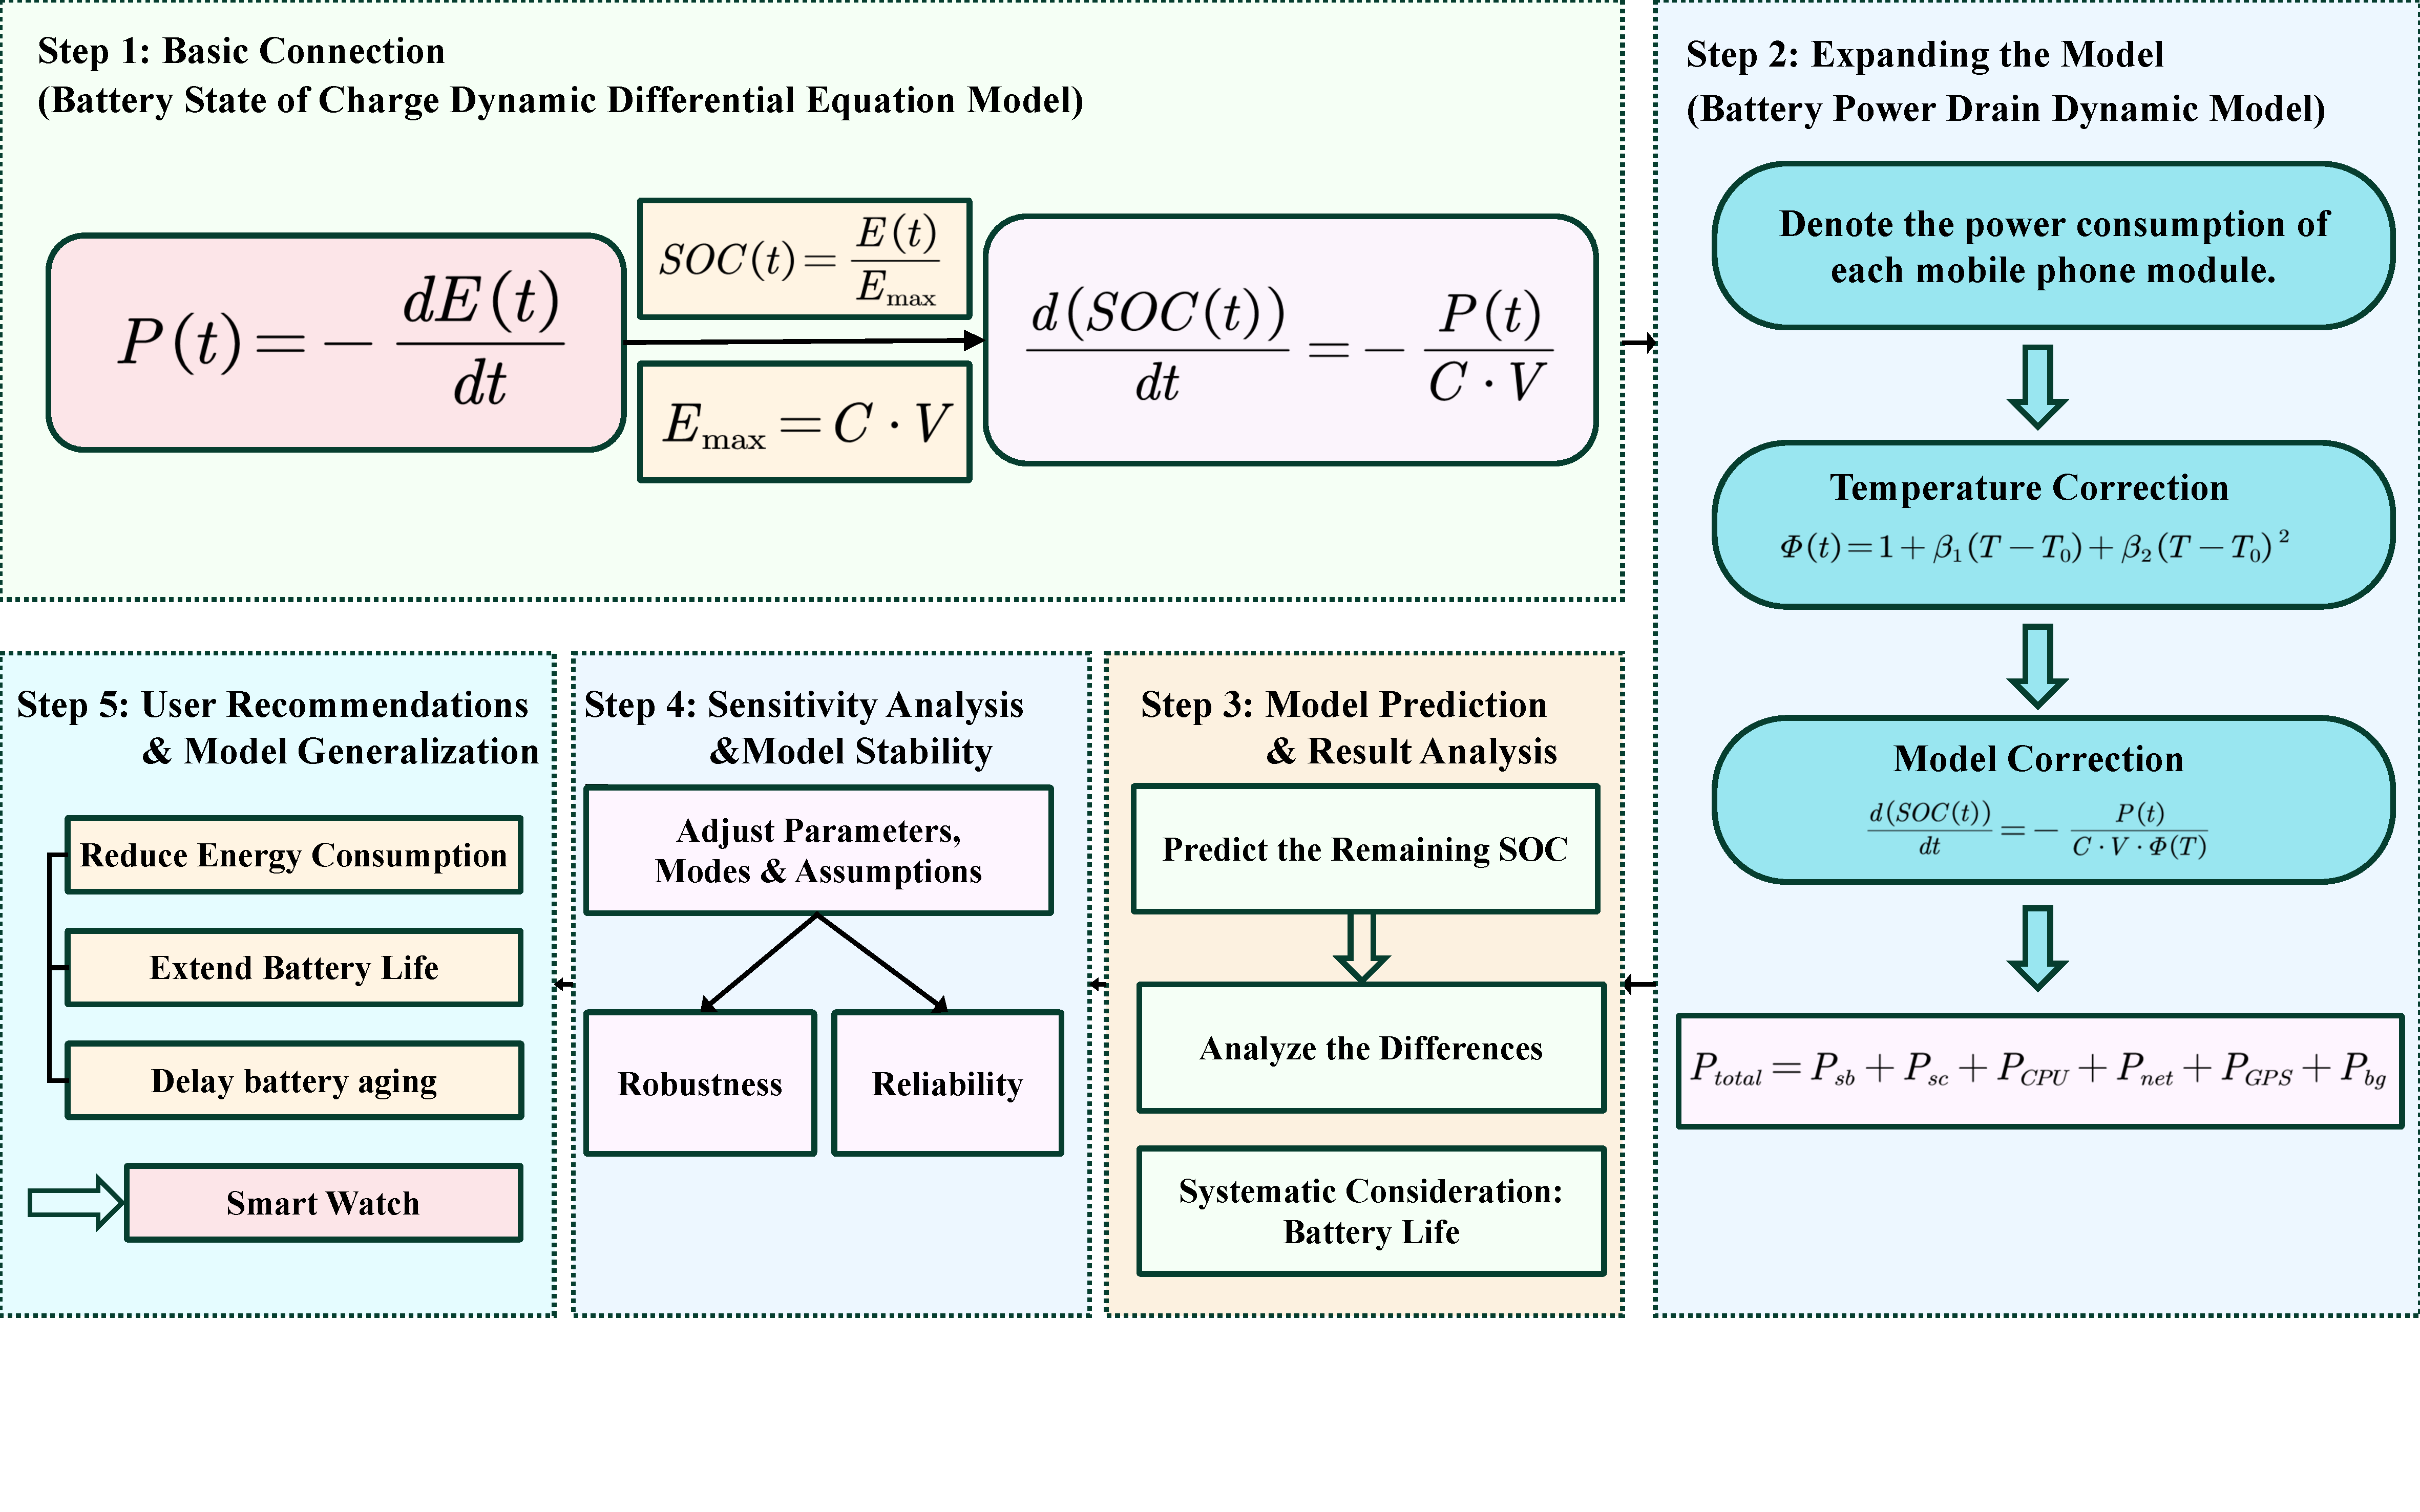
\includegraphics[width=1.05\textwidth,trim=0cm 6.5cm 0cm 0cm, 
%clip]{figures/2026美赛流程图.pdf}
%\caption{问题一分析流程图}
%\label{fig:问题一分析}
%\end{figure}

\begin{figure}[h!]
	\centering
	% trim = 左边裁剪 下边裁剪 右边裁剪 上边裁剪（单位：cm）
	% clip 表示启用裁剪功能
	\vspace{0cm}
	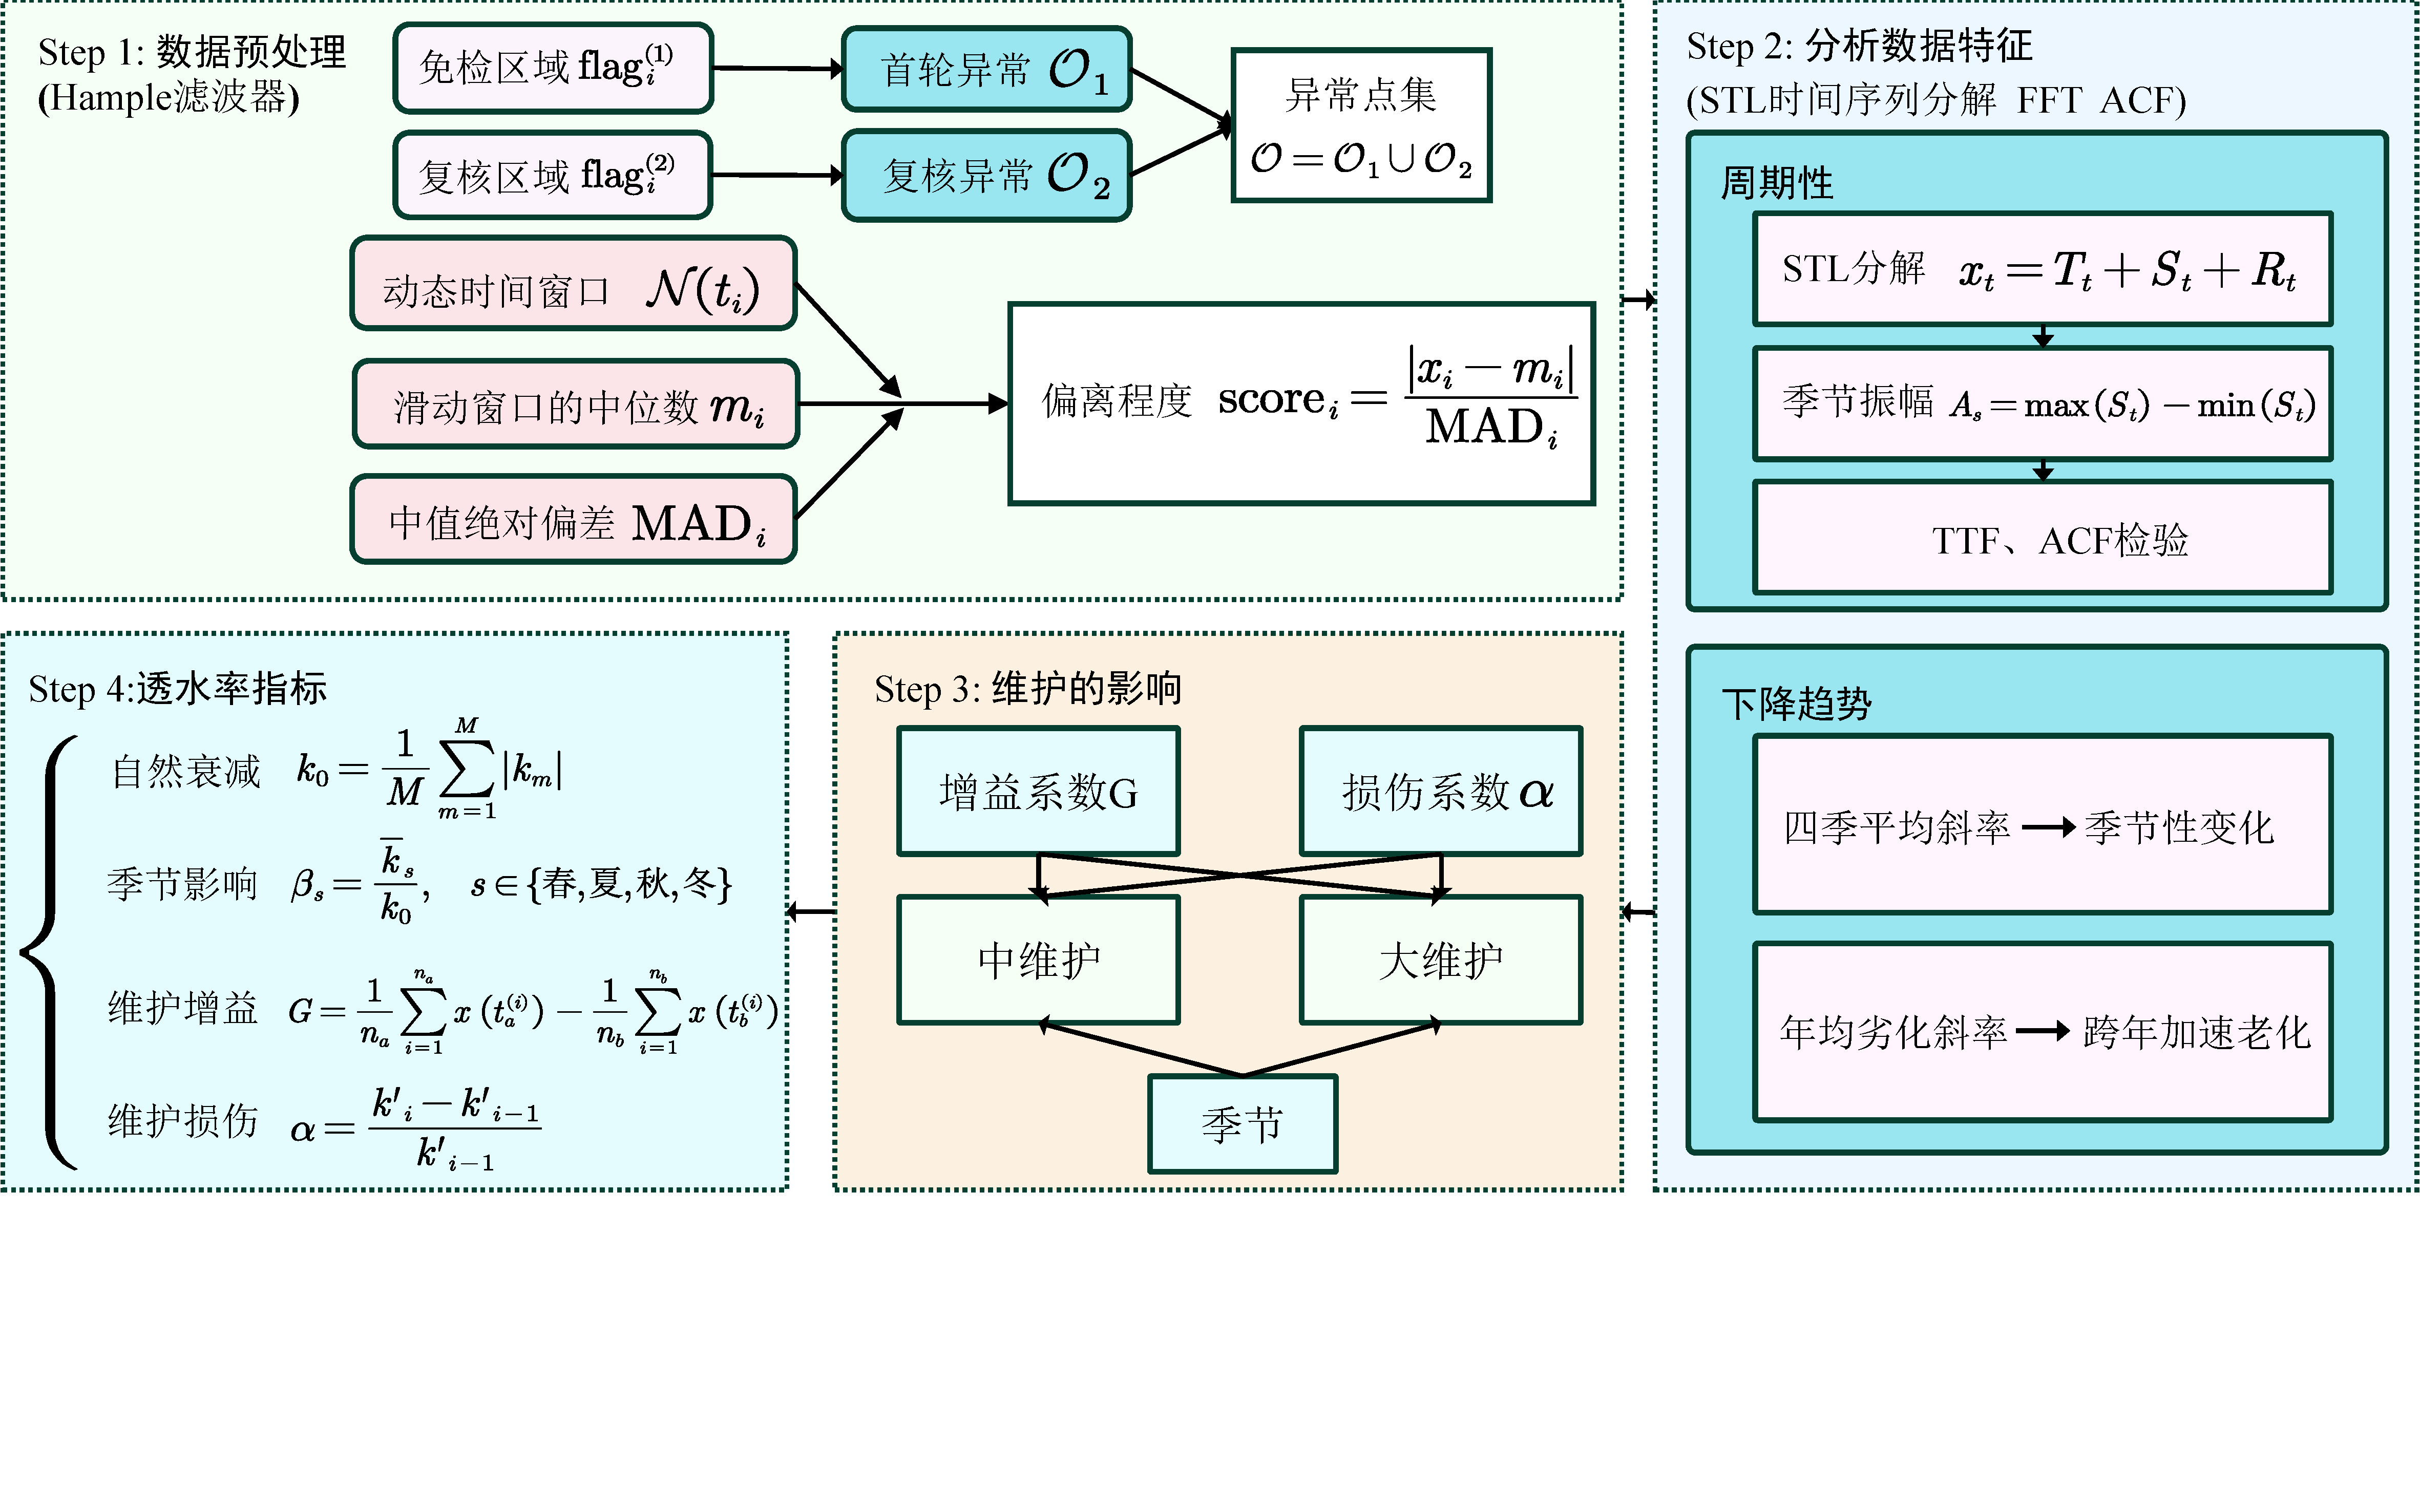
\includegraphics[
	width=1\textwidth,
	trim=0cm 10cm 0cm 0cm, 
	clip
	]{figures/问题一分析.pdf}
	\caption{问题一分析流程图}
	\label{fig:问题一分析}
\end{figure}

首先对问题进行拆分，问题一主要有4方面的要求：对数据预处理、分析数据的特征以及规律、探究维护类型对透水率的影响、给出影响透水率的重要指标。以下为解决4个需求的方法分析：

\begin{enumerate}[label=\bfseries\arabic*.,leftmargin=40pt]
	\item \textbf{数据预处理：}
	
	对于缺失值，按成因分为两类处理：在中维护和大维护期间，因维护操作导致的数据缺失，不进行填补，以保留原始无记录状态；非维护期间的缺失，若位于数据起始阶段则直接剔除，其他如适配传感器临时故障等因素造成的短期缺失，采用多段线性插值填补，既能保持时间序列的整体趋势，又不会引入明显偏差。
	
	对于异常值，我们需要在保留维护引起的阶跃变化的前提下，剔除其他随机异常波动。首先依据维护事件标记保护期，将保护期内数据直接视为正常值且不参与检测；随后对非保护期数据使用 Hampel 滤波器逐点统计检测并标记异常点。对非维护期出现的短期连续异常，结合现场记录判断是否为持续性堵塞或故障，确属异常的追加标记。全部标记完成后，对异常点使用线性插值做替换处理。
	
	
	\item \textbf{分析数据特征：}
	
	由于想知道数据在时间维度上的性质，我们通过STL时间序列拆分得到了过滤器透水率的季节振幅，从而得到透水率的周期规律，随后通过FFT与ACF指标验证了规律的正确性。
	
	将下降趋势规律拆分为一年内的季节性变化和年与年之间的周期变化。通过STL时间序列拆分得到的季节振幅，结合设置的季节影响算子，得出透水率在不同季节的下降规律。又通过对比不同年份同一季节的下降趋势可以得到过滤器随着时间推移下降趋势的规律。

	
	\item \textbf{维护类型对透水率的影响：}
	
	在附件1的数据中看出小维护对透水率的改善有限，又因小维护成本不计，于是我们主要研究中维护与大维护对透水率的影响。通过引入维护增益与维护损伤系数判断每次中维护与大维护对过滤器性能的影响。
	
	\item \textbf{造成透水率变化的指标：}
	
	针对过滤器对透水率的的自然衰减、季节对透水率的影响、维护对过滤器造成的不可逆的损伤、维护对透水率的增加4个关键影响，分别建立基准劣化率、季节影响算子、维护损伤系数、维护增益4个指标。指标可以通过附件1的数据拟合、列式计算得到。
	
\end{enumerate}

\vspace*{-20pt}
\subsection{问题二分析}	
\begin{figure}[h!]
	\centering
	% trim = 左边裁剪 下边裁剪 右边裁剪 上边裁剪（单位：cm）
	% clip 表示启用裁剪功能
	\vspace*{-15pt}
	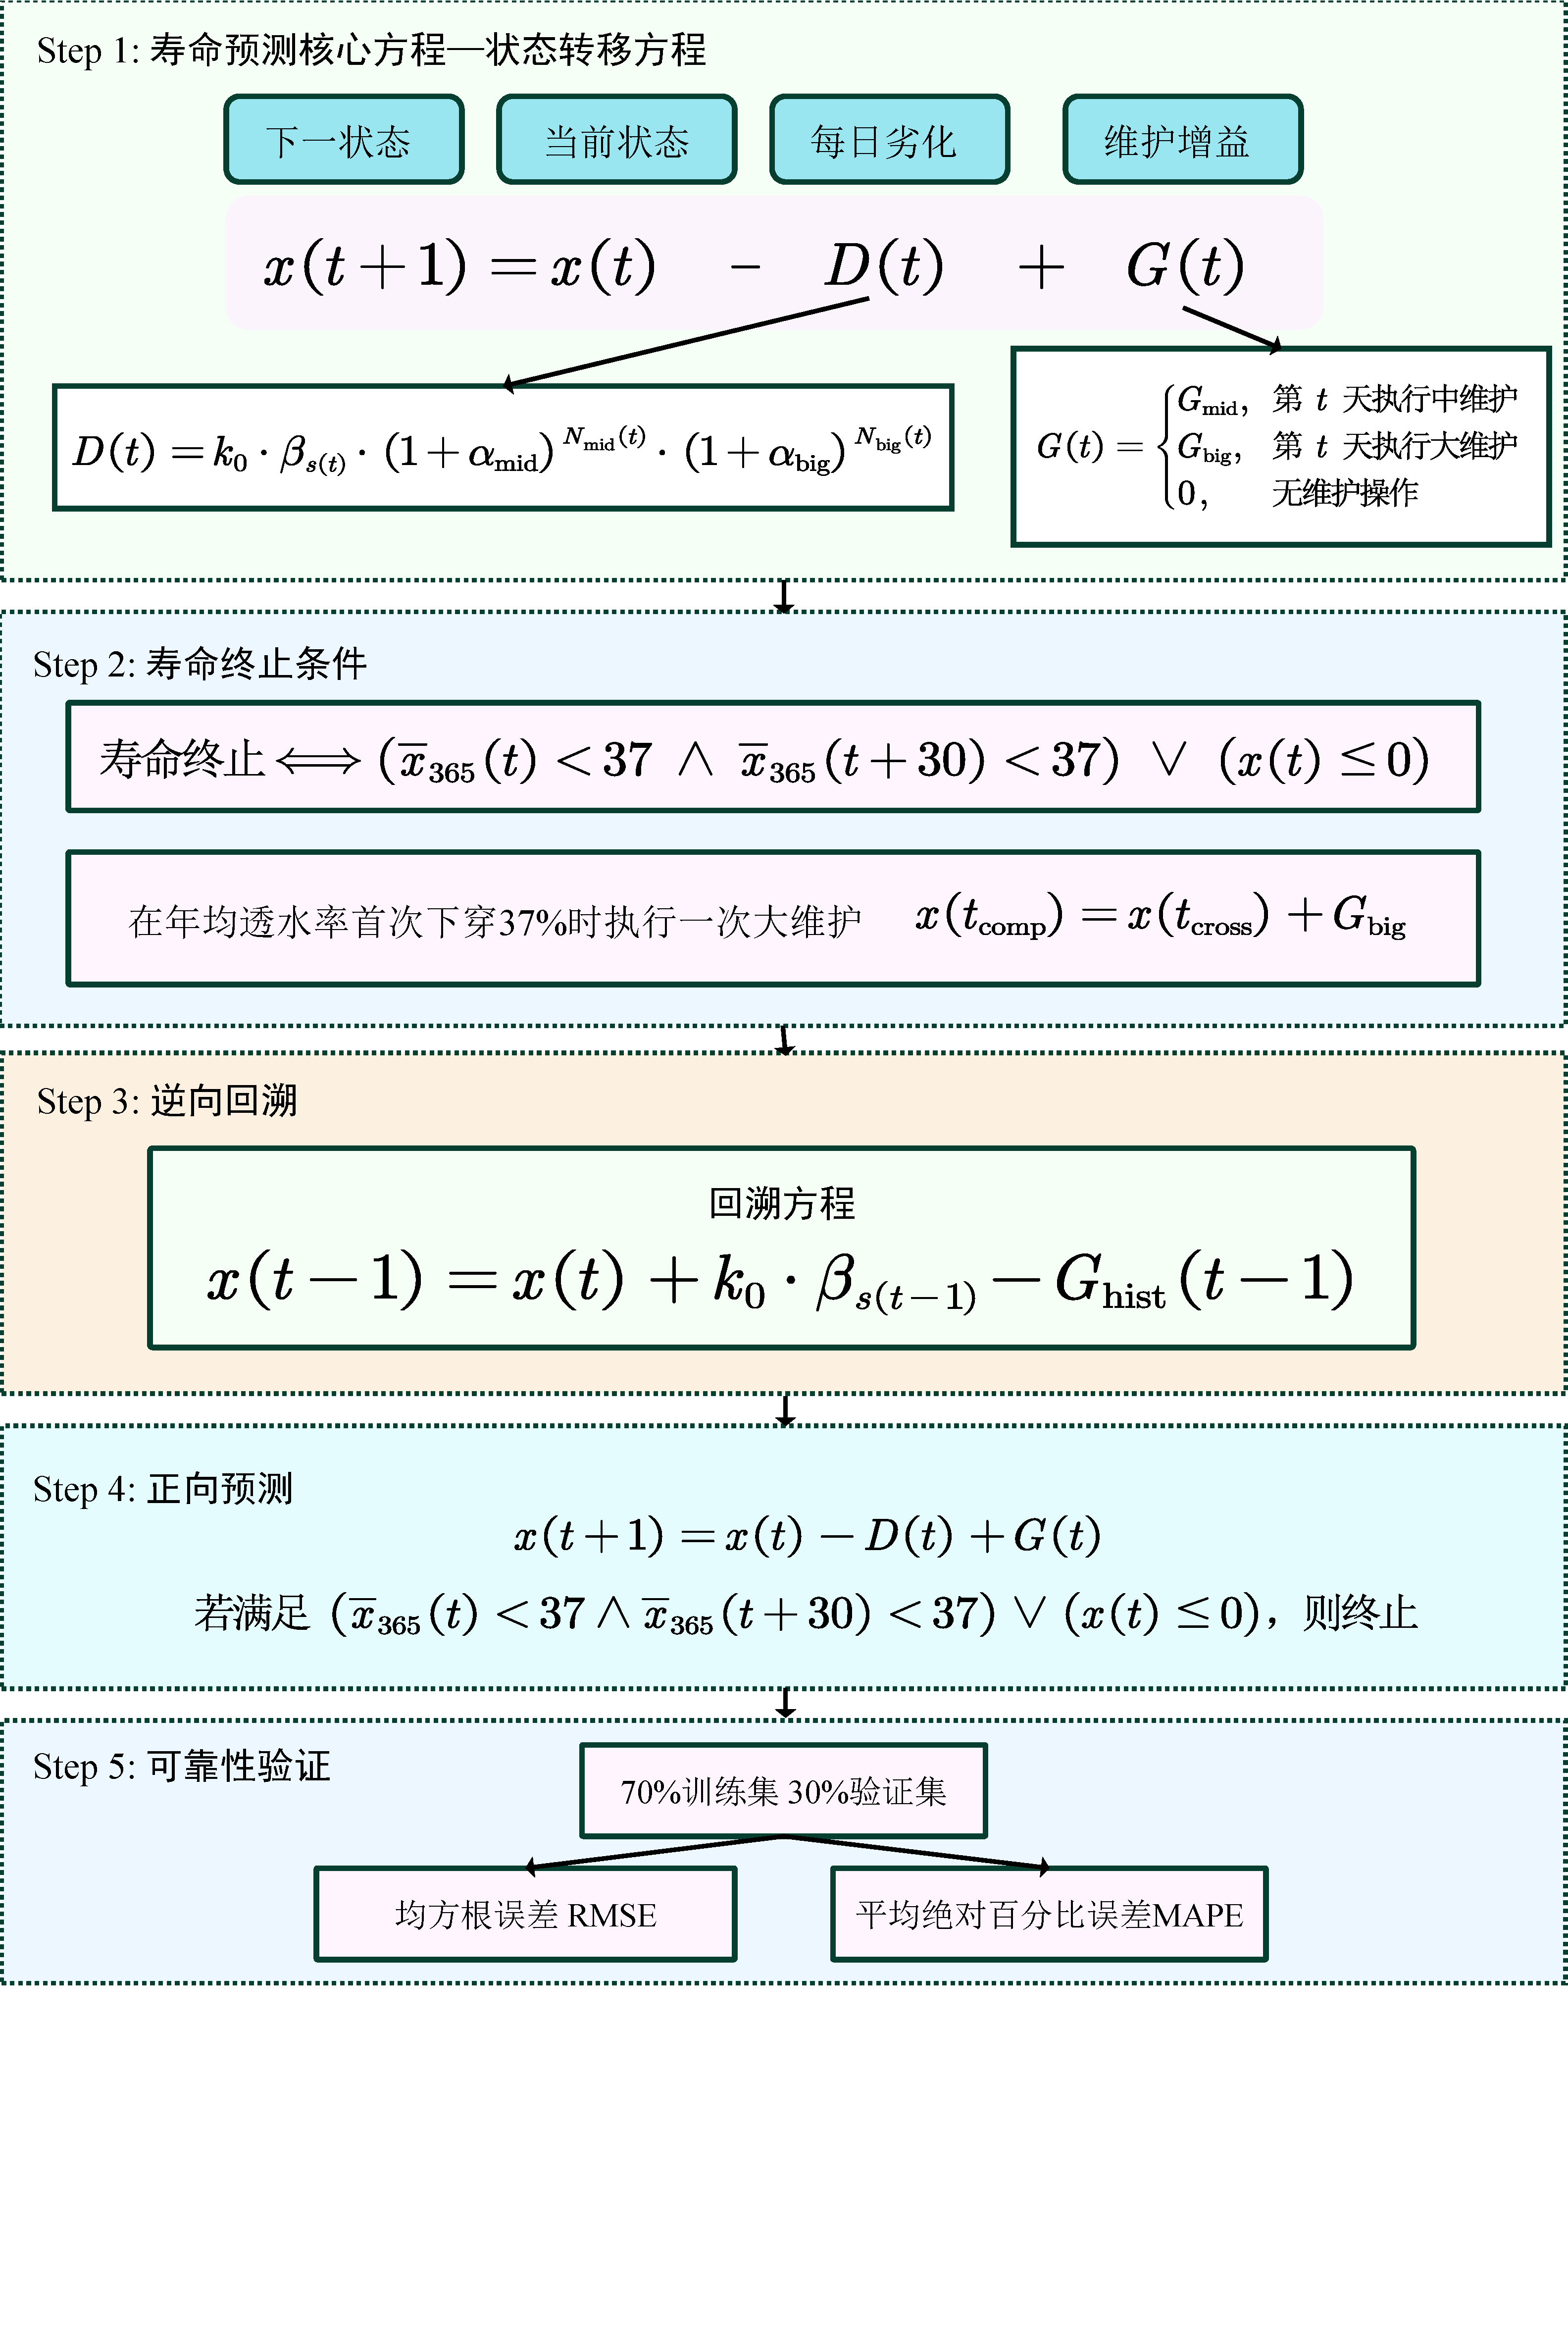
\includegraphics[
	width=0.63\textwidth,
	trim=0cm 12cm 0cm 0cm, 
	clip
	]{figures/问题二分析.pdf}
	\caption{问题二分析流程图}
	\label{fig:问题二分析}
\end{figure}

为了综合考虑过滤器的性能的自然下降、季节对过滤器性能的影响、维护对透水率的影响，将第一问中的4个指标相互关联，并纳入第二问的寿命预测模型，即状态转移方程。将模型分别套用至每个过滤器，得到每台过滤器的各项指标以及固定维护规律。当过去以年的平均透水率低于37时，且维护后一个月以内又下降至37及以下时，判定为过滤器寿命终止。随后建立逆向回溯方程，回溯过滤器在出厂状态时的透水率，再正向预测至寿命终止。最后给出10台过滤器的寿命预测结果，设置训练集与测试集并使用RMSE与MAPE进行模型可靠性验证。

\subsection{问题三分析}

基于前两问对过滤器劣化的规律以及维护对透水率的影响，建立优化模型：

\begin{enumerate}[label=\bfseries\arabic*.,leftmargin=40pt]
	\item \textbf{优化函数}：通过预测模型预测出的一个过滤器从开始使用到寿命终止的一个完整使用周期，随后计算出整个使用周期的成本，再通过一个使用周期的成本换算到一年的成本。以年均成本最小为优化函数，
	\item \textbf{决策变量}：考虑到透水率下降速率与距上次维护时间均影响维护需求，设立中维护时间间隔阈值 $T_{\text{mid}}$ 与退化速率触发阈值 $r_{\text{th}}$ 两个决策变量，实现固定间隔与状态响应的混合调度；考虑到过滤器长期运行后性能严重衰减，设立大维护时间间隔阈值 $T_{\text{big}}$ 决策变量，控制大维护执行频率。
	
	\item \textbf{约束条件}：考虑到过滤器实际运行的物理约束，从四个方面建立约束条件：透水率始终为正、365天滑动平均透水率不低于37、透水率演化服从第二问状态转移方程、维护触发逻辑由决策变量按规则控制。
\end{enumerate}

最后根据本题动态系统约束是非线性的、维护行为会导致状态跳变、目标函数不可解析表达的特点，选择使用遗传算法制定维护策略。

\subsection{问题四分析}

改变过滤器购买价格与维护成本验证维护策略的稳健性，也就是对过滤器购买价格与维护成本进行敏感性分析。于是需要设置题目给的过滤器价格与维护价格波动。为了量化建立的策略在新参数下的表现，可以设损失率$\delta$为固定策略不变，年均成本相对于新成本下重新优化所得年均成本的偏差比例，并用它进行敏感性分析。


%%%%%%%%%%%%%%%%%%%%%%%%%%%%%%%%%%%%%%%%%%%%%%%%%%%%%%%%%%%%% 

\section{模型假设}

\begin{enumerate}[label=\arabic*.]
	\item 假设小维护对透水率改善有限且成本可忽略不计。附件数据显示小维护频率高但单次效果微弱，且题目明确其成本可忽略，因此我们只研究中维护与大维护的影响。
	
	\item 假设维护操作在维护日当天立即生效。实际维护后透水率会在较短时间内恢复，为简化模型，假设增益在维护当日一次性完成。
	
	\item 假设季节对透水率下降速率的影响按月离散变化，不同月份对应不同的影响系数。季节变化对过滤器性能的影响在月份交界处变化显著，且数据难以支持连续函数拟合，故采用离散跳变的季节算子进行建模。
	
	\item 假设未来气候与运行条件保持稳定。缺乏未来年份的环境预测数据，故假设历史规律可外推。
\end{enumerate}

%%%%%%%%%%%%%%%%%%%%%%%%%%%%%%%%%%%%%%%%%%%%%%%%%%%%%%%%%%%%% 

\section{符号说明}
\begin{table}[h!]
	\centering
	\renewcommand{\arraystretch}{1.5}
	\setlength{\tabcolsep}{30pt}
%	\caption{符号说明}
	\label{tab:符号说明}
	\begin{tabular}{lcc}
		\toprule[1.5pt]
		\textbf{符号} & \textbf{说明} & \textbf{单位} \\
		\midrule
		\rowcolor{LightBlue}
		$x(t)$ & 第 $t$ 天的透水率 & -- \\
		$\bar{x}_{365}(t)$ & 前365天滑动平均透水率 & -- \\
		\rowcolor{LightBlue}
		$k_0$ & 基准劣化率 & --/天 \\
		$\beta_s$ & 季节影响算子 & -- \\
		\rowcolor{LightBlue}
		$G_{\text{mid}}$ & 中维护瞬时增益 & -- \\
		$G_{\text{big}}$ & 大维护瞬时增益 & -- \\
		\rowcolor{LightBlue}
		$\alpha_{\text{mid}}$ & 中维护损伤系数 & -- \\
		$\alpha_{\text{big}}$ & 大维护损伤系数 & -- \\
		\rowcolor{LightBlue}
		$N_{\text{mid}}(t)$ & 截至第 $t$ 天的中维护累计次数 & -- \\
		$N_{\text{big}}(t)$ & 截至第 $t$ 天的大维护累计次数 & -- \\
		\rowcolor{LightBlue}
		$A_s$ & 季节振幅 & -- \\
		$T_t$ & STL分解趋势分量 & -- \\
		\rowcolor{LightBlue}
		$S_t$ & STL分解季节分量 & -- \\
		$R_t$ & STL分解残差分量 & -- \\
		\rowcolor{LightBlue}
		$C_{\text{purchase}}$ & 过滤器购买价格 & 万元 \\
		$c_{\text{mid}}$ & 单次中维护成本 & 万元 \\
		\rowcolor{LightBlue}
		$c_{\text{big}}$ & 单次大维护成本 & 万元 \\
		$L$ & 过滤器总寿命 & 年 \\
		\rowcolor{LightBlue}
		$J$ & 年均成本 & 万元/年 \\
		$T_{\text{mid}}$ & 中维护时间间隔阈值 & 天 \\
		\rowcolor{LightBlue}
		$T_{\text{big}}$ & 大维护时间间隔阈值 & 天 \\
		$r_{\text{th}}$ & 退化速率触发阈值 & --/天 \\
		\rowcolor{LightBlue}
		$\delta$ & 损失率 & \% \\
		\bottomrule[1.5pt]
	\end{tabular}
\end{table}

%%%%%%%%%%%%%%%%%%%%%%%%%%%%%%%%%%%%%%%%%%%%%%%%%%%%%%%%%%%%% 

\section{问题一的模型的建立和求解}

我们围绕数据预处理、数据特征与规律分析、维护类型对透水率的影响探究，以及关键影响指标识别四个方面，分别开展建模与求解工作。

\subsection{利用Hampel滤波器进行数据预处理}

针对工业污水过滤器透水率数据存在随机异常波动、缺失值、维护引发阶跃变化且采样间隔不均匀的特点，采用带维护事件标记的改进自适应Hampel滤波器完成数据预处理。该方法基于动态时间窗口与绝对中位差构建稳健识别规则，采用两阶段检测策略，既能剔除随机噪声与异常点，又能完整保留维护操作带来的真实阶跃信号，适配透水率长期衰减、受季节与维护共同影响的监测场景\upcite{1}。

\subsubsection{异常点的判断方法}

我们采用动态时间窗口$\mathcal{N}(t_i)$对数据进行分段处理，以时间替代固定点数来划分判断该点是正常点或异常点的半径：
\begin{equation}
	\mathcal{N}(t_i) = \left\{ x_j \mid |t_j - t_i| \leq \Delta T_{\max},\ j \neq i \right\},
\end{equation}
其中：$x_j$ 为时间点 $t_j$ 处的透水率测量值，$\Delta T_{\max} = 72$ 小时为最大时间搜索半径。该设计使滤波器能够适应数据采样间隔不均匀的实际工况。

为保证窗口内有足够的点来判定该点是否为异常值，设置窗口内需要至少有5个点，即添加最低约束：
\begin{equation}
	|\mathcal{N}(t_i)| \geq N_{\min},\quad N_{\min} = 5.
\end{equation}

采用滑动窗口的中位数$m_i$作为该点正常值的基准：
\begin{equation}
	m_i = \text{median}\left\{ x_j \mid j \in \mathcal{N}(t_i) \right\}.
\end{equation}

采用中值绝对偏差$\text{MAD}_i$来作为基于正常值的波动范围：
\begin{equation}
	\text{MAD}_i = \text{median}\left\{ |x_j - m_i| \mid j \in \mathcal{N}(t_i) \right\}.
\end{equation}

使用异常评分函数$score_i$判断偏离正常值的尺度：
\begin{equation}
	\text{score}_i = \frac{|x_i - m_i|}{\text{MAD}_i}.
\end{equation}

与传统Hampel滤波器不同，我们不使用 $1.4826$ 缩放系数，直接以原始MAD作为尺度估计，使异常判定标准更为严格，避免透水率数据中异常波动的漏检。

\subsubsection{两阶段自适应检测策略}

维护操作引发的透水率阶跃变化属于真实物理信号，不应被滤波器误判为异常。为此，本文构建两阶段自适应检测策略，在保护维护信号的同时识别真正的异常点。

基于维护事件标记，定义第一阶段免检区域为维护日与其之后的24小时：
\begin{equation}
	\text{flag}_i^{(1)} =
	\begin{cases}
		1, & t_i \in \text{维护日} \cup (\text{维护日} + 24\text{h}) \\
		0, & \text{其他}.
	\end{cases}
\end{equation}

第一轮检测仅对免检区域外的数据点进行异常判定：
\begin{equation}
	\mathcal{O}_1 = \left\{ i \mid \text{score}_i > T,\ \text{flag}_i^{(1)} = 0,\ |\mathcal{N}(t_i)| \geq N_{\min} \right\},\quad T = 3.
\end{equation}

为避免第一轮异常点对后续检测造成干扰，采用线性插值对其进行临时填充，得到中间序列：
\begin{equation}
	\tilde{x}_i =
	\begin{cases}
		x_i, & i \notin \mathcal{O}_1, \\
		\text{interp}(t_i), & i \in \mathcal{O}_1.
	\end{cases}
\end{equation}

第一轮检测中被免检的点，即在维护后24小时内的点，也可能有异常点，需进行第二轮复核。第二轮检测区域为：
\begin{equation}
	\text{flag}_i^{(2)} =
	\begin{cases}
		1, & t_i \in (\text{维护日} + 24\text{h}) \setminus \text{维护日}, \\
		0, & \text{其他}.
	\end{cases}
\end{equation}

为确保复核的独立性，第二轮检测的参考窗口排除维护日当天的数据点：
\begin{equation}
	\mathcal{N}^{(2)}(t_i) = \left\{ j \mid |t_j - t_i| \leq \Delta T_{\max},\ j \neq i,\ \text{flag}_j^{(\text{day})} = 0 \right\}.
\end{equation}

第二轮异常检测规则为：
\begin{equation}
	\mathcal{O}_2 = \left\{ i \mid \text{score}_i^{(2)} > T,\ \text{flag}_i^{(2)} = 1,\ |\mathcal{N}^{(2)}(t_i)| \geq N_{\min} \right\}.
\end{equation}

最终异常点集合取两轮检测结果的并集：
\begin{equation}
	\mathcal{O} = \mathcal{O}_1 \cup \mathcal{O}_2.
\end{equation}

\subsubsection{滤波后的缺失值处理}

最后对异常值进行处理，使用线性插值填补，能保留时间序列趋势，不会引入大偏差：
\begin{equation}
	\hat{x}_i = x_{i_L} + \frac{x_{i_R} - x_{i_L}}{t_{i_R} - t_{i_L}} \cdot (t_i - t_{i_L}).
	\label{线性插值}
\end{equation}

其中 $\hat{x}_i$ 为待插值点 $t_i$ 处的估计值，$t_{i_L}$ 和 $t_{i_R}$ 分别为 $t_i$ 前后最近有效数据点的时间坐标，$x_{i_L}$ 和 $x_{i_R}$ 为对应时间点的透水率测量值，$\frac{x_{i_R} - x_{i_L}}{t_{i_R} - t_{i_L}}$ 为两点间的斜率。

维护日及维护后24小时的原始缺失值保持为NaN，不进行插值，最终处理得到的值为：
\begin{equation}
	x_i^{\text{clean}} =
	\begin{cases}
		\text{NaN}, & i \in \text{维护期} \cap \text{原始缺失}, \\
		\hat{x}_i, & i \in \mathcal{O} \cup \text{原始缺失}, \\
		x_i, & \text{其他}.
	\end{cases}
\end{equation}

对非维护期内存在的缺失值，同样采用(\ref{线性插值})式的线性插值方法进行填补。

\subsubsection{数据预处理结果}

采用改进的自适应 Hampel 滤波器对原始透水率数据进行清洗，有效剔除异常波动并填补缺失值。以设备 A5 和 A6 为例，清洗前后的透水率序列对比如图 \ref{fig:A5对比} 和图 \ref{fig:A6对比} 所示：

\begin{figure}[h!]
	\centering
	\subcaptionbox{过滤器A5原始透水率序列\label{fig:A5清洗前}}%
	{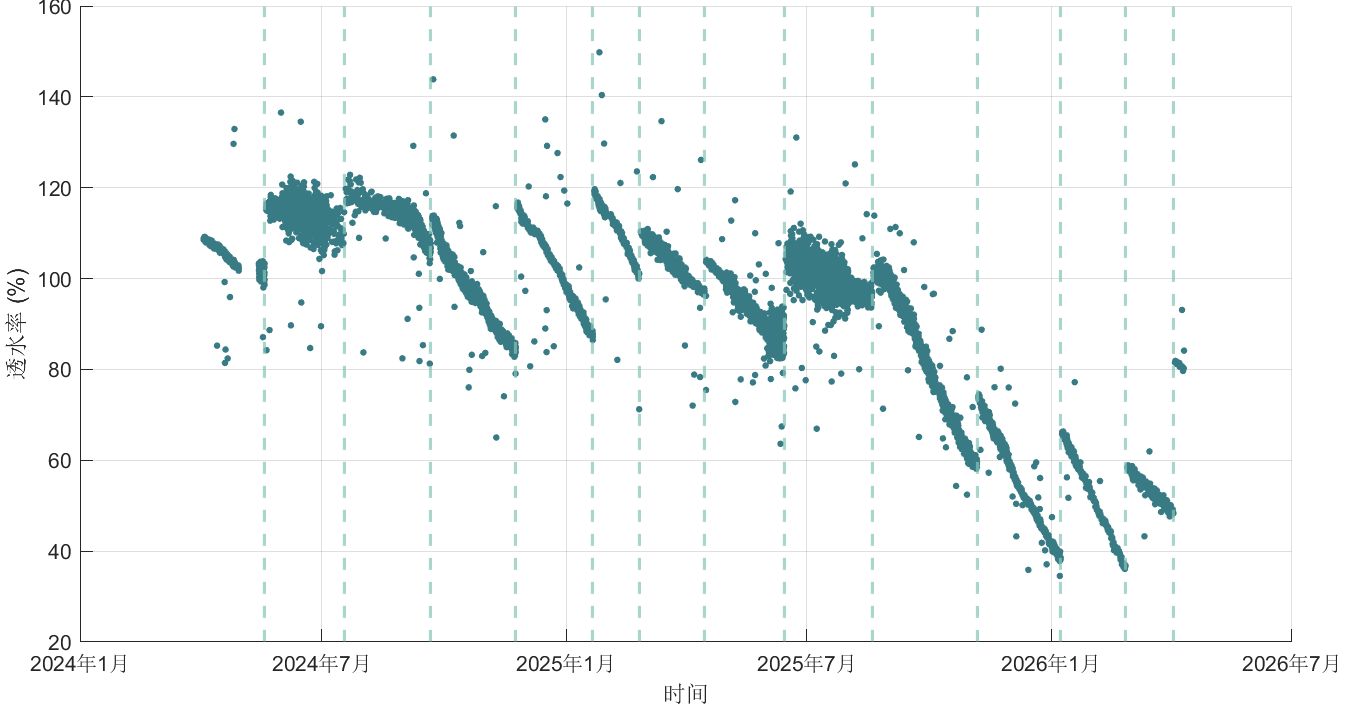
\includegraphics[width=.5\textwidth]{figures/A5清洗前.png}}%
	\subcaptionbox{过滤器A5清洗后透水率序列\label{fig:A5清洗后}}%
	{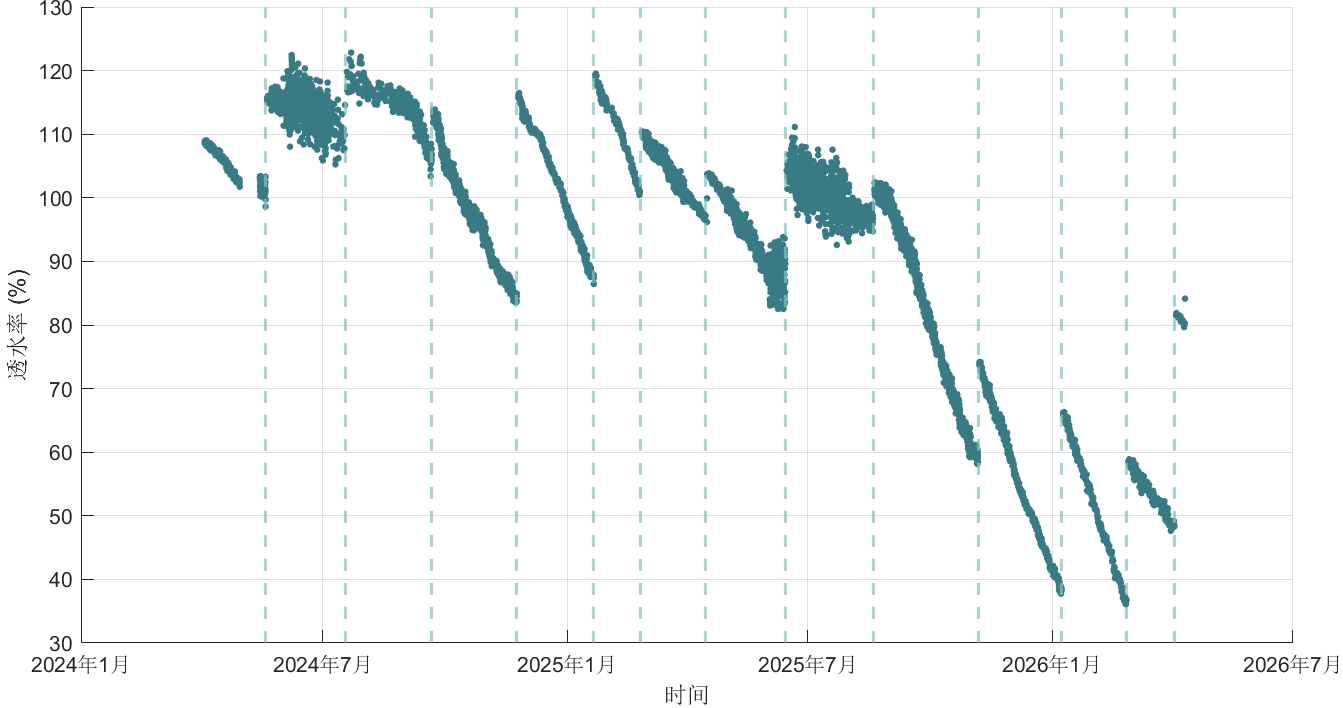
\includegraphics[width=.5\textwidth]{figures/A5清洗后.png}}
	\caption{过滤器A5数据清洗前后对比}
	\label{fig:A5对比}
\end{figure}

\begin{figure}[h!]
	\centering
	\subcaptionbox{过滤器A6原始透水率序列\label{fig:A6清洗前}}%
	{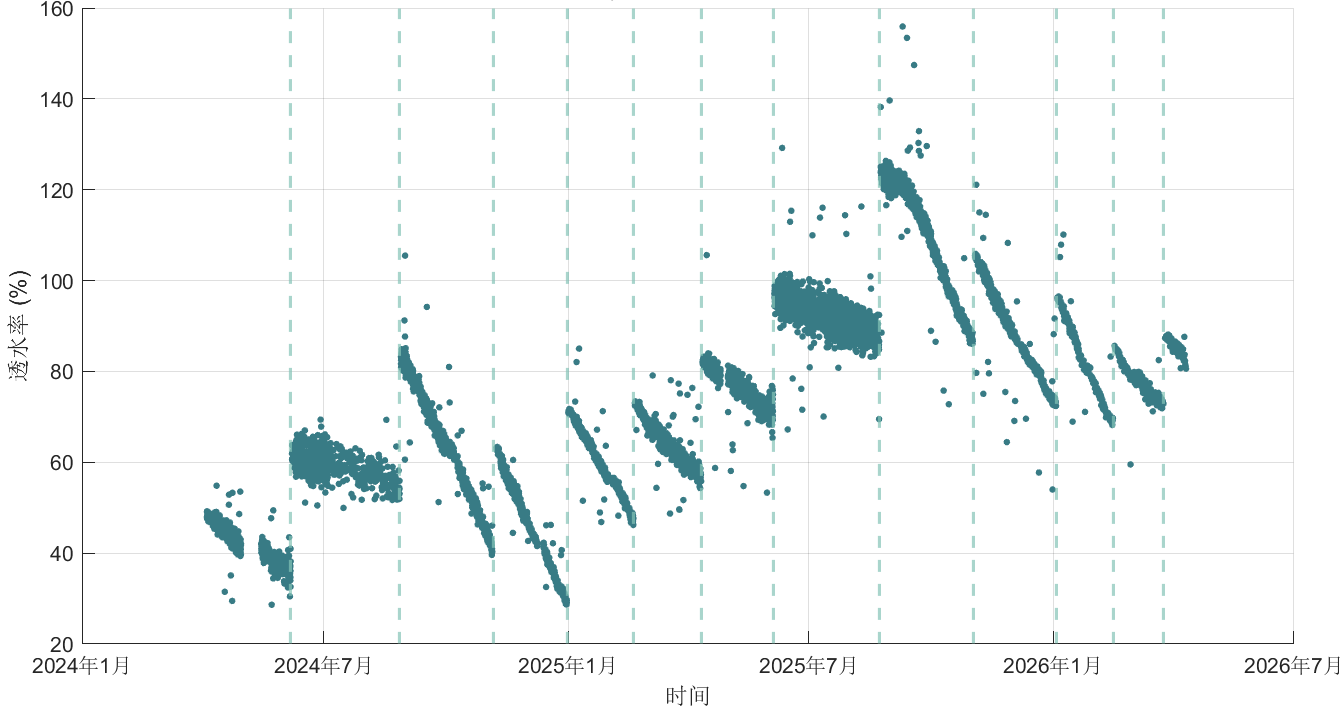
\includegraphics[width=.5\textwidth]{figures/A6清洗前.png}}%
	\subcaptionbox{过滤器A6清洗后透水率序列\label{fig:A6清洗后}}%
	{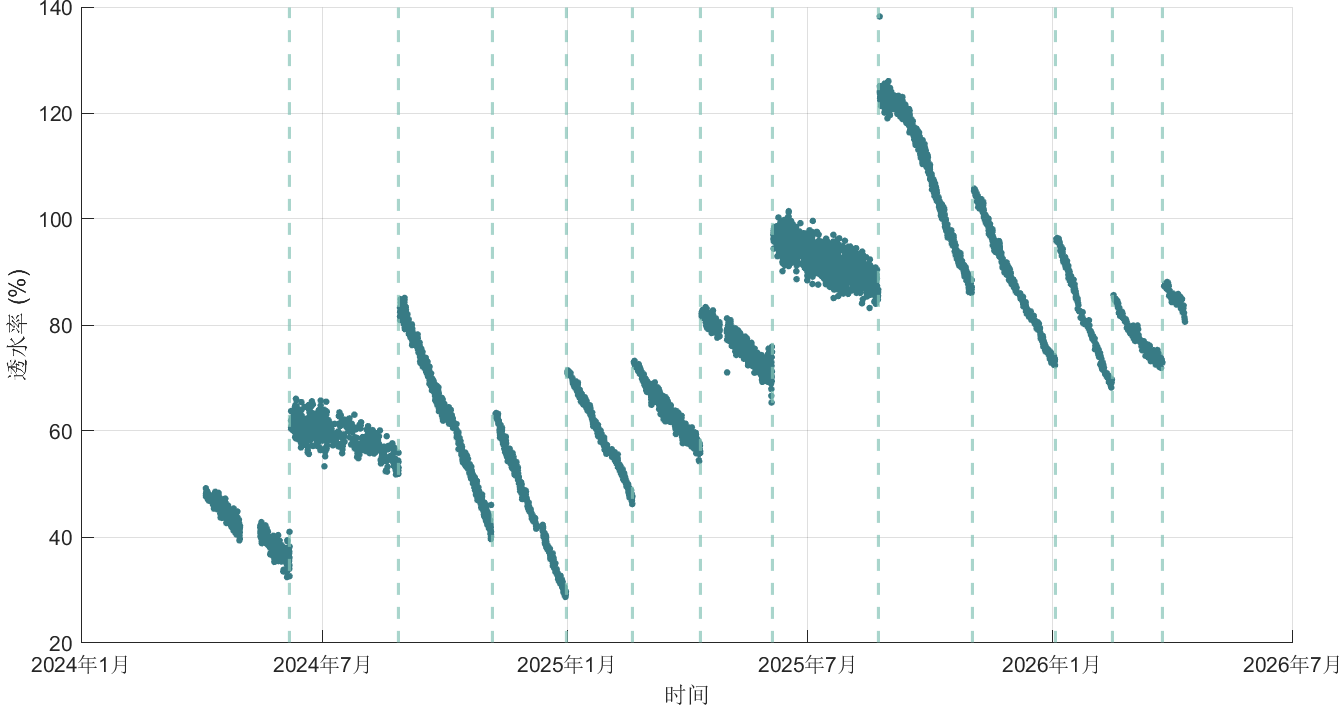
\includegraphics[width=.5\textwidth]{figures/A6清洗后.png}}
	\caption{过滤器A6数据清洗前后对比}
	\label{fig:A6对比}
\end{figure}

从图中看出，经过改进的自适应 Hampel 滤波处理后，透水率序列中的异常跳变点被有效剔除，缺失值通过线性插值得到合理填补，序列整体趋势更加平滑、连续且稳定，为后续的劣化特性分析与寿命预测模型构建提供了高质量的数据基础。

\subsection{分析数据特征}

接下来分别分析数据的周期性、下降趋势规律。

\subsubsection{数据的周期性}
透水率作为反映过滤器性能与状态的核心指标，其变化受环境温度、水质条件等季节性因素影响显著。为识别数据中隐含的周期波动，采用\textbf{STL（Seasonal-Trend decomposition using Loess）分解法}对每台过滤器的日均透水率序列进行拆解\upcite{2}。

STL方法基于局部加权回归，将原始序列分解为三个可解释的分量：
\begin{equation}
	x_t = T_t + S_t + R_t,
	\label{STL}
\end{equation}
其中$x_t$是第$t$日的透水率，$T_t$是趋势分量，反映过滤器长期老化导致的透水率单调下降，$S_t$是季节分量，反映以一年为周期的规律性波动，$R_t$是残差分量，代表随机噪声或未捕获的细微扰动。三个分量的具体构造方式如下：

\begin{itemize}
	\item \textbf{趋势项 $T_t$}：采用滑动平均对原始数据做平滑处理，滤除短期波动和周期波动，体现曲线的的大致走向，表示过滤器因老化导致的透水率逐年下滑趋势。
	
	\item \textbf{季节项 $S_t$}：从原始数据中减去趋势项得到，随后对每个周期位置分别取平均，形成一个固定的年度波形。为使季节分量在各周期之间可比，进一步对该波形进行中心化处理，使其在一个完整周期内的均值为零，即$\sum_{t=1}^{365}S_t = 0$。最终结果呈现为每年重复的波动形态。
	
	\item \textbf{残差项 $R_t$}：定义为原始序列减去趋势项与季节项后的剩余部分，即$R_t = x_t - T_t - S_t$，代表随机噪声或细微扰动。
\end{itemize}

上述分解过程通过MATLAB内置函数\texttt{trenddecomp}实现，调用格式为：
\begin{lstlisting}[language=Matlab, basicstyle=\small\ttfamily]
	[trend, seasonal, residual] = trenddecomp(daily_per_full, 'stl', 365);
\end{lstlisting}
其中\texttt{daily\_per\_full}为日均透水率序列，\texttt{'stl'}指定STL分解方法，\texttt{365}把一年设置为周期参数。

我们选择过滤器A2来展示STL的分析结果，即(\ref{STL})式的4个变量：

\newpage

\begin{figure}[h!]
	\centering
	\vspace*{0pt}
	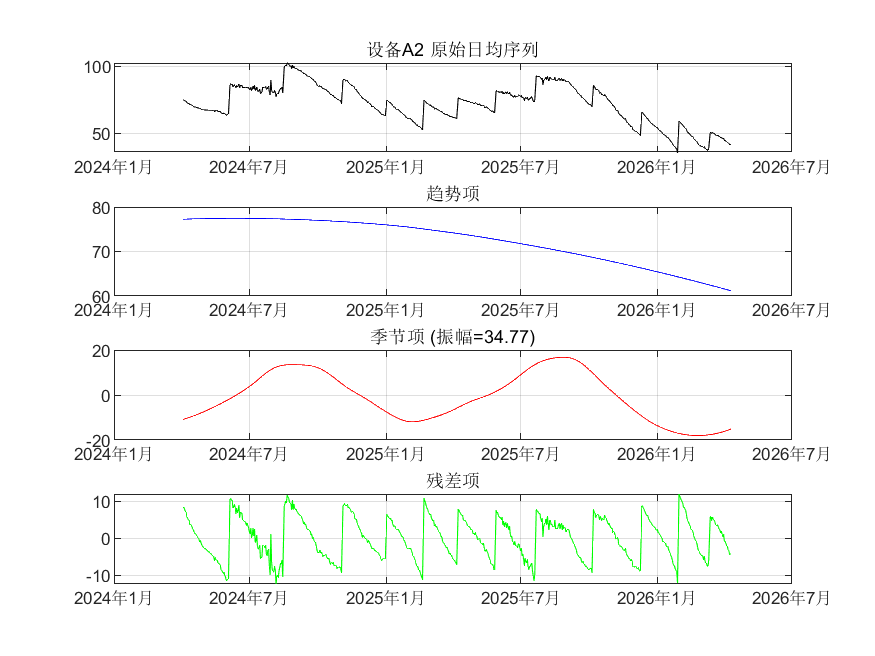
\includegraphics[width=0.7\textwidth,trim=0cm 0.7cm 0cm 0.5cm,clip]{figures/A2.png}
	\caption{A2过滤器的STL参数}
	\label{fig:A2}
\end{figure}

\vspace*{-10pt}
从图~\ref{fig:A2}中可以看出：
\begin{itemize}
	\item 原始序列呈现出明显的“冬季低、夏季高”的年度波动形态
	\item 趋势分量剥离季节影响后，透水率整体呈缓慢下降趋势，符合过滤器老化规律
	\item 季节分量展现出稳定的周期性波形，每年重复相似的变化模式
	\item 残差分量幅值较小且随机分布，表明分解充分提取了主要信号
\end{itemize}

为量化季节效应的强度，我们用季节分量$S_t$定义季节振幅$A_s$：

\vspace*{-10pt}
\begin{equation}
	A_s = \max(S_t) - \min(S_t)
\end{equation}

它代表一年内纯季节因素引起的透水率最大波动幅度。

接着挑选了A1-A5过滤器重点分析季节性分量以及季节振幅以得到周期性规律。
\begin{figure}[h!]
	\centering
	\vspace*{0pt}
	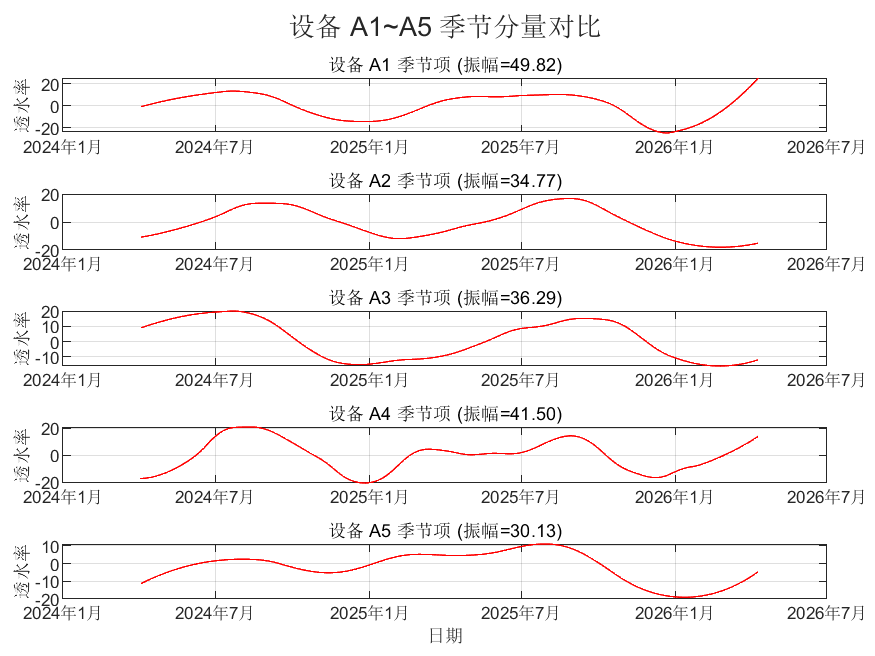
\includegraphics[width=0.7\textwidth,trim=0cm 0.5cm 0cm 0.7cm,clip]{figures/季节振幅.png}
	\caption{过滤器A1-A5的季节分量变化}
	\label{fig:季节振幅图}
\end{figure}

由图~\ref{fig:季节振幅图}看出季节分量以一年为周期进行波动，说明过滤器的透水率存在以一年为周期的波动特征。10台过滤器的季节振幅结果如表~\ref{tab:季节振幅表}所示。

\begin{table}[h!]
	\centering
	\renewcommand{\arraystretch}{1.5}
	\caption{各过滤器季节振幅统计}
	\label{tab:季节振幅表}
	\begin{tabular}{lcccccccccc}
		\toprule[1.5pt]
		过滤器 & A1 & A2 & A3 & A4 & A5 & A6 & A7 & A8 & A9 & A10 \\
		\midrule
		\rowcolor{LightBlue}
		振幅$A_s$ & 49.82 & 41.07 & 45.18 & 37.81 & 32.94 & 42.75 & 27.09 & 31.46 & 35.01 & 51.87 \\
		\bottomrule[1.5pt]
	\end{tabular}
\end{table}

10台过滤器的季节振幅介于27.09至51.87之间，平均值为38.52。注意到不同过滤器对季节变化的敏感程度存在差异，比如A10、A1等过滤器振幅较大，说明其性能受季节影响更为显著，A7、A5等过滤器振幅相对较小，季节干扰相对平缓。

随后采用\textbf{快速傅里叶变换（FFT）}对去趋势后的序列进行频域分析，并绘制\textbf{自相关函数（ACF）}图，以验证结论。

\begin{figure}[h!]
	\centering
	\renewcommand{\arraystretch}{0.8}
	\subcaptionbox{过滤器A1透水率FFT功率谱\label{fig:FFT}}%
	{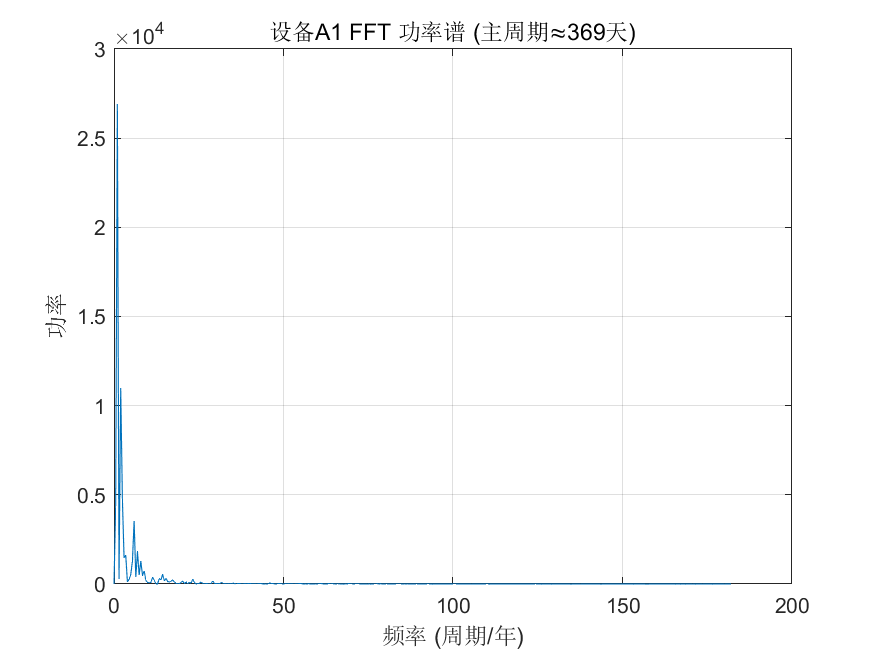
\includegraphics[width=.5\textwidth]{figures/FFT.png}}%
	\subcaptionbox{过滤器A1透水率自相关函数\label{fig:ACF}}%
	{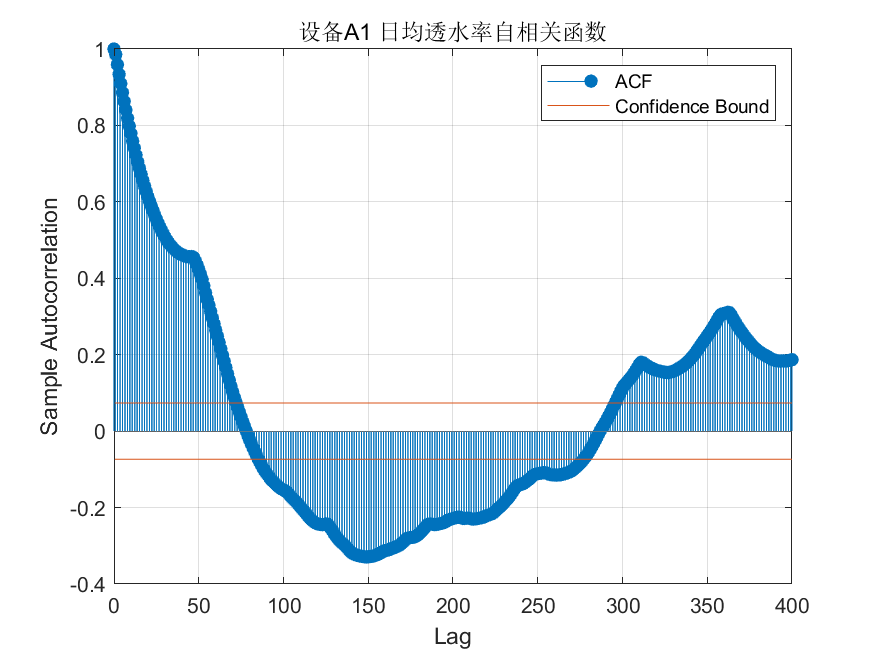
\includegraphics[width=.5\textwidth]{figures/ACF.png}}
	\caption{过滤器A1透水率序列的周期性分析（FFT与ACF）}
	\label{fig:FFTACF}
	\renewcommand{\arraystretch}{1.5}
\end{figure}

由图~\ref{fig:FFTACF}，过滤器A1的FFT功率谱与自相关函数（ACF）共同验证了其日均透水率的周期性：
\begin{itemize}
	\item 由图~\ref{fig:FFT}，FFT功率谱图以频率为横轴、功率强度为纵轴，识别序列中的主导周期成分。图中在频率$x=\frac{1}{369}$处出现显著主峰，对应主周期约369天，接近一年的周期，且无其他高频强周期，表明透水率存在强烈的年周期性波动。
	\item 由图~\ref{fig:ACF}，自相关函数图以滞后阶数（天）为横轴、样本自相关系数为纵轴，用于衡量序列与其滞后项的相关性。图中在滞后约350-380天处呈现明显的正相关峰值，且超出置信界，印证了透水率序列存在约一年的周期波动；同时，在0-150天左右，自相关系数从1快速衰减，反映了序列的短期强自相关性，说明透水率变化具有连续性，受之前透水率影响显著。
\end{itemize}

综合STL分解、频谱分析与自相关检验，得到过滤器的透水率变化是以年为周期的。


\subsubsection{下降趋势规律}
我们以时间为分隔，研究一年之间的下降趋势规律，还有年与年之间的下降变化规律。前者的变化主要来源于季节的影响，后者的变化主要来源于维护与过滤器自然老化的影响。
\paragraph{一年内季节下降规律}

将各维护间隔内的日均劣化斜率按季节归类，分别计算春、夏、秋、冬四季的平均斜率。第 $m$ 个维护间隔内的劣化斜率 $k_m$ 通过对该时段内的日均透水率序列进行线性拟合得到：
\begin{equation}
	k_m = \frac{n \sum_{i=1}^{n} t_i x_i - \sum_{i=1}^{n} t_i \sum_{i=1}^{n} x_i}{n \sum_{i=1}^{n} t_i^2 - \left( \sum_{i=1}^{n} t_i \right)^2},
\end{equation}
其中 $t_i$ 为间隔内的第 $i$ 天，$x_i$ 为对应日的透水率，$n$ 为该间隔内的有效天数。

将各间隔按其时间中点的月份归入对应季节，分别计算各季节内斜率的平均值：
\begin{equation}
	\bar{k}_s = \frac{1}{M_s} \sum_{m \in \mathcal{S}_s} k_m, \quad s \in \{\text{春},\text{夏},\text{秋},\text{冬}\},
	\label{eq:ksbar}
\end{equation}
其中 $\mathcal{S}_s$ 为属于季节 $s$ 的间隔索引集合，$M_s$ 为集合大小。

经过计算，春、夏、秋、冬四季的平均斜率结果如表~\ref{tab:一年内}所示。

\begin{table}[H]
	\centering
	\setlength{\tabcolsep}{4pt}
	\renewcommand{\arraystretch}{1.2}
	\caption{各过滤器四季劣化斜率}
	\label{tab:一年内}
	\begin{tabular}{ccccc}
		\toprule
		\textbf{过滤器} & \textbf{春季斜率} & \textbf{夏季斜率} & \textbf{秋季斜率} & \textbf{冬季斜率} \\
		\midrule
		\rowcolor{LightBlue}
		A1 & -0.2694 & -0.1718 & -0.4886 & -0.4828 \\
		A2 & -0.2512 & -0.1628 & -0.4997 & -0.5248 \\
		\rowcolor{LightBlue}
		A3 & -0.2063 & -0.1620 & -0.5862 & -0.6186 \\
		A4 & -0.1854 & -0.1589 & -0.5063 & -0.4766 \\
		\rowcolor{LightBlue}
		A5 & -0.2445 & -0.1342 & -0.5245 & -0.5588 \\
		A6 & -0.2754 & -0.1024 & -0.5919 & -0.5745 \\
		\rowcolor{LightBlue}
		A7 & -0.2471 & -0.1518 & -0.5606 & -0.5064 \\
		A8 & -0.2891 & -0.1275 & -0.6277 & -0.5128 \\
		\rowcolor{LightBlue}
		A9 & -0.2268 & -0.1183 & -0.4454 & -0.5487 \\
		A10 & -0.2737 & -0.1576 & -0.6338 & -0.6250 \\
		\midrule
		\textbf{平均} & \textbf{-0.2469} & \textbf{-0.1447} & \textbf{-0.5465} & \textbf{-0.5429} \\
		\bottomrule
	\end{tabular}
\end{table}

从四季平均斜率来看，夏季劣化最慢，平均斜率为-0.1447单位/天；秋季和冬季劣化最快，平均斜率分别为-0.5465和-0.5429单位/天，约为夏季的3.8倍；春季介于两者之间，平均斜率为-0.2469单位/天。该规律符合流体的物理特性：夏季水温高、水体粘度低，流体通过滤芯的阻力较小，故透水率下降缓慢；秋冬季水温降低、水体粘度增大，同时水中悬浮物浓度升高、微生物活性变化，导致滤芯堵塞加速，透水率快速衰减。

\begin{figure}[h!]
	\centering
	% trim = 左边裁剪 下边裁剪 右边裁剪 上边裁剪（单位：cm）
	% clip 表示启用裁剪功能
	\vspace{0cm}
	\hspace*{-7pt}
	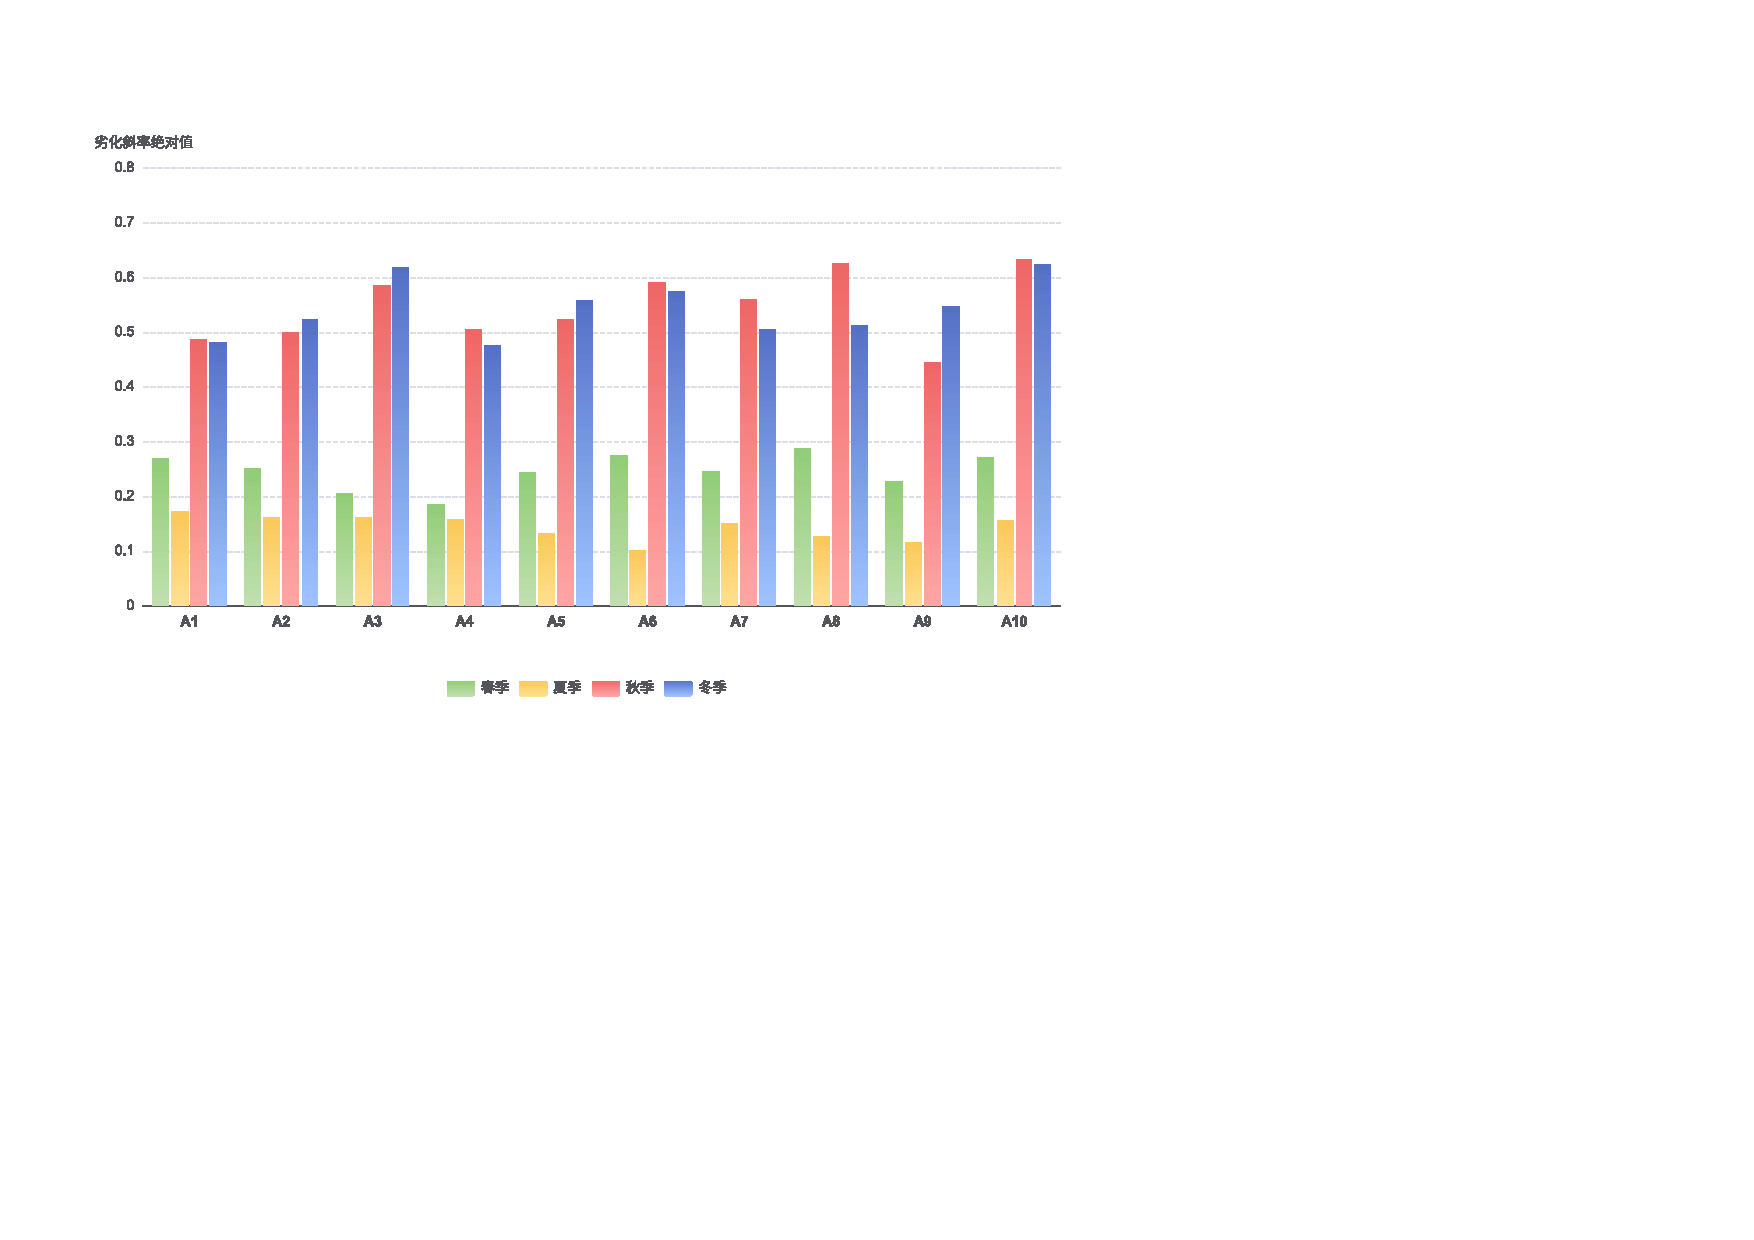
\includegraphics[
	width=.95\textwidth,
	trim=0cm 0cm 0cm 0cm, 
	clip
	]{figures/各过滤器四季劣化斜率对比.pdf}
	\caption{各过滤器四季劣化斜率对比}
	\label{fig:各过滤器四季劣化斜率对比}
\end{figure}

由图~\ref{fig:各过滤器四季劣化斜率对比}，10台过滤器的透水率劣化速率呈现出高度一致的季节性特征：秋冬季劣化速率最快，斜率绝对值显著高于春夏季；夏季劣化速率最慢，劣化进程明显放缓；春季则表现为过渡性特征。

\paragraph{跨年份下降规律}

为考察过滤器性能随使用年限的退化趋势，按年度统计各过滤器的年均劣化斜率，结果如表~\ref{tab:跨年份}所示。

\begin{table}[H]
	\centering
	\setlength{\tabcolsep}{4pt}
	\renewcommand{\arraystretch}{1.2}
	\caption{各过滤器年度劣化斜率}
	\label{tab:跨年份}
	\begin{tabular}{ccccccccccc}
		\toprule
		\textbf{年度} & \textbf{A1} & \textbf{A2} & \textbf{A3} & \textbf{A4} & \textbf{A5} & \textbf{A6} & \textbf{A7} & \textbf{A8} & \textbf{A9} & \textbf{A10} \\
		\midrule
		\rowcolor{LightBlue}
		2024.4-2025.3 & -0.2919 & -0.3138 & -0.3586 & -0.3268 & -0.3131 & -0.3800 & -0.3155 & -0.3489 & -0.3476 & -0.3901 \\
		2025.4-2026.4 & -0.3790 & -0.3870 & -0.3710 & -0.3365 & -0.3882 & -0.3977 & -0.3834 & -0.3801 & -0.3385 & -0.4111 \\
		\bottomrule
	\end{tabular}
\end{table}

对比两个年度数据，除A3和A4外，其余8台过滤器的劣化斜率绝对值均呈现不同程度的增大，即透水率下降速度随时间加快。其中A2从-0.3138增至-0.3870，增幅达23.3\%；A5从-0.3131增至-0.3882，增幅达24.0\%；A10从-0.3901增至-0.4111，增幅为5.4\%。这表明随着使用年限增加，过滤器的自然老化与维护累积损伤共同作用，导致过滤器加速老化。

综合上述分析，透水率下降呈现出季节周期性与跨年度加速老化的特征。季节周期性为维护时间提供了建议：因为冬天透水率下降快，可以考虑在冬季维护。跨年度加速老化的特征帮助工厂制定维护或更换方案。



\subsection{维护类型对透水率的影响}

维护操作对透水率产生两方面影响：一是维护后透水率的瞬时提升幅度，即维护增益；二是维护对后续劣化速度的长期影响，即维护损伤。我们分别分析增益与损伤对中维护与大维护的作用。

\subsubsection{维护增益分析}

维护增益定义为维护前后各3天透水率均值之差：
\[
	G = \frac{1}{n_{\text{after}}} \sum_{i=1}^{n_{\text{after}}} x(t_{\text{after}}^{(i)}) - \frac{1}{n_{\text{before}}} \sum_{i=1}^{n_{\text{before}}} x(t_{\text{before}}^{(i)}),
\]
其反映单次维护的即时恢复能力。各过滤器中维护与大维护的平均增益统计结果如表~\ref{tab:维护增益}所示。

\begin{table}[H]
	\centering
	\setlength{\tabcolsep}{4pt}
	\renewcommand{\arraystretch}{1.2}
	\caption{各过滤器维护增益统计}
	\label{tab:维护增益}
	\begin{tabular}{cccc}
		\toprule
		\textbf{过滤器} & \textbf{中维护增益} & \textbf{大维护增益} & \textbf{增益差值} \\
		\midrule
		\rowcolor{LightBlue}
		A1 & 16.40 & 7.72 & 8.69 \\
		A2 & 12.48 & 12.82 & -0.35 \\
		\rowcolor{LightBlue}
		A3 & 12.34 & 10.28 & 2.07 \\
		A4 & 16.25 & -- & -- \\
		\rowcolor{LightBlue}
		A5 & 13.19 & 3.96 & 9.23 \\
		A6 & 18.22 & 16.66 & 1.57 \\
		\rowcolor{LightBlue}
		A7 & 10.43 & 16.59 & -6.16 \\
		A8 & 10.70 & -- & -- \\
		\rowcolor{LightBlue}
		A9 & 13.95 & 12.89 & 1.05 \\
		A10 & 11.03 & 8.12 & 2.91 \\
		\midrule
		\textbf{平均} & \textbf{13.50} & \textbf{11.13} & \textbf{2.37} \\
		\bottomrule
	\end{tabular}
\end{table}

从整体水平来看，10台过滤器中维护平均增益为13.50，大维护平均增益为11.13，中维护短期恢复效果平均高出约2.37个透水率单位。中维护增益普遍较高且稳定，介于10.43至18.22之间；大维护增益波动较为剧烈，介于3.96至16.66之间。A1、A5等过滤器的大维护增益远低于中维护，反映出大维护时过滤器可能已处于深度劣化状态，即使彻底清洗也难以恢复到较高水平。值得注意的是，A2和A7的大维护增益反超中维护，这可能是因为大维护时机恰好处于透水率极低点，且大维护清洗更为彻底，使得恢复幅度反而更大。

结合现实分析，中维护以清除近期附着物为主，能快速释放被堵孔道，因而瞬时增益较高。大维护虽能更深度清理，但其透水率已大幅衰减，可恢复的绝对空间减小，导致维护增益反而不大。

\begin{figure}[h!]
	\centering
	% trim = 左边裁剪 下边裁剪 右边裁剪 上边裁剪（单位：cm）
	% clip 表示启用裁剪功能
	\vspace{0cm}
	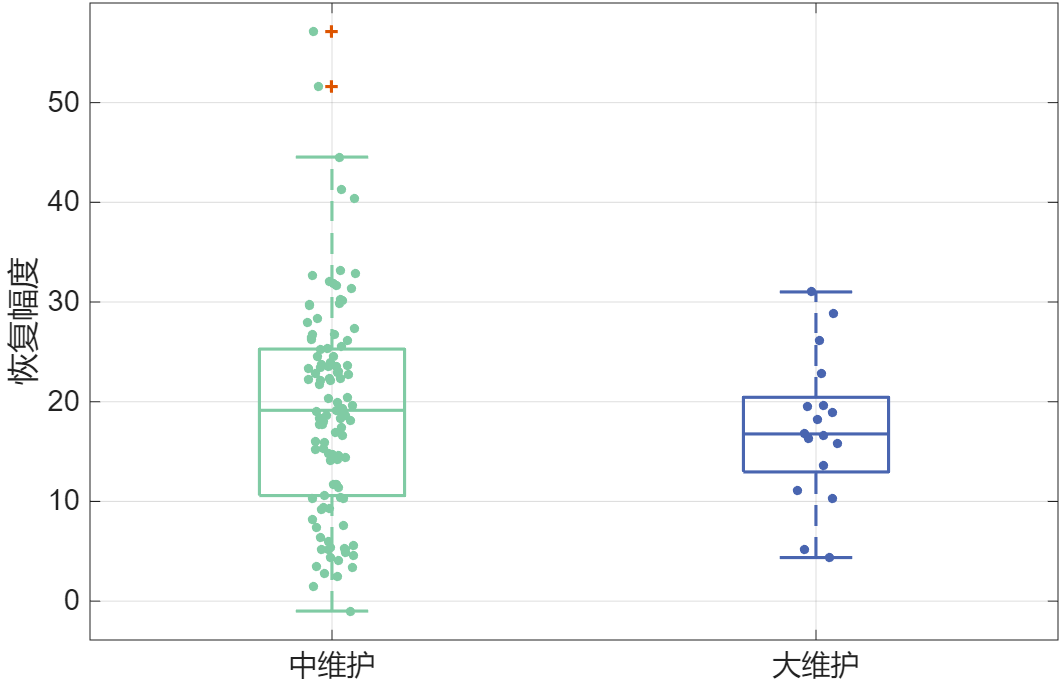
\includegraphics[
	width=.85\textwidth,
	trim=0cm 0cm 0cm 0cm, 
	clip
	]{figures/不同维护类型恢复幅度对比.png}
	\caption{不同维护类型恢复幅度对比}
	\label{fig:不同维护类型恢复幅度对比}
\end{figure}

由图~\ref{fig:不同维护类型恢复幅度对比}，中维护的透水率恢复幅度整体略高于大维护，其中位数约为 20\%，且分布更分散，存在多个超过 40\% 的高恢复值；大维护的恢复幅度则更集中稳定，中位数约为17\%，整体波动范围较小，二者共同反映出中维护在部分工况下的瞬时恢复能力更强，而大维护的恢复效果更具一致性。

\subsubsection{维护损伤分析}

纳入维护损伤系数 $\alpha$ 量化维护操作对过滤器劣化速度的影响，用剔除季节因素后相邻段纯净劣化率的相对变化率来表示，先剔除季节因素：
\[
k'_i = \frac{|k_i|}{\beta_{s(i)}},
\]
其中 $k_i$ 为第 $i$ 段的有量纲斜率，$\beta_{s(i)}$ 为该段所属季节的季节算子\( \beta_s = \frac{\bar{k}_s}{k_0}, s \in \{\text{春},\text{夏},\text{秋},\text{冬}\} \)，$k_0$取斜率的绝对值后平均\(k_0 = \frac{1}{M} \sum_{m=1}^{M} |k_m|\)。则损伤系数定义为相邻段纯净劣化率的相对变化率：
\[
	\alpha = \frac{k'_{i} - k'_{i-1}}{k'_{i-1}},
\]
正值表示劣化加速，负值表示劣化减缓。我们把负值都填充为0，因为维护之后的一段时间理论上透水率下降应该更快，在模型中负值属于不合理的值。各过滤器损伤系数统计如表~\ref{tab:维护损伤}所示。

\begin{table}[H]
	\centering
	\setlength{\tabcolsep}{4pt}
	\renewcommand{\arraystretch}{1.2}
	\caption{各过滤器维护损伤系数统计}
	\label{tab:维护损伤}
	\begin{tabular}{cccc}
		\toprule
		\textbf{过滤器} & \textbf{中维护损伤系数} & \textbf{大维护损伤系数} & \textbf{损伤系数差值} \\
		\midrule
		\rowcolor{LightBlue}
		A1 & 0.0554 & 0.1166 & -0.0613 \\
		A2 & 0.1967 & 0.0000 & 0.1967 \\
		\rowcolor{LightBlue}
		A3 & 0.1262 & 0.0890 & 0.0372 \\
		A4 & 0.2270 & 0.0000 & 0.2270 \\
		\rowcolor{LightBlue}
		A5 & 0.0178 & 0.0000 & 0.0178 \\
		A6 & 0.0181 & 0.1773 & -0.1593 \\
		\rowcolor{LightBlue}
		A7 & 0.2082 & 0.0000 & 0.2082 \\
		A8 & 0.2494 & 0.0000 & 0.2494 \\
		\rowcolor{LightBlue}
		A9 & 0.0281 & 0.3995 & -0.3714 \\
		A10 & 0.0570 & 0.7481 & -0.6911 \\
		\midrule
		\textbf{平均} & \textbf{0.1184} & \textbf{0.1531} & \textbf{-0.0347} \\
		\bottomrule
	\end{tabular}
\end{table}

中维护损伤系数平均值为0.1184，大维护损伤系数平均值为0.1531，二者差异不大。值得注意的是，过滤器A4、A8由于没有大维护记录，大维护损伤系数为0；过滤器A2、A5、A7的大维护损伤原始值为负，截断后变为0，意味着大维护往往能使维护后的斜率变得更平缓，即大维护能有效减缓短期劣化速度，但一段时间后老化速率可能会增加。而中维护由于清洗不彻底，残留垢层可能导致局部污堵加速，使得损伤系数多为正值。大维护的真实损伤主要体现在永久峰值衰减上，而非劣化速度的加速。

\subsubsection{季节对维护增益的影响}

季节因素对维护增益具有显著影响。按维护发生所在季节统计中维护的平均增益，结果如表~\ref{tab:中维护季节}所示。

\begin{table}[H]
	\centering
	\setlength{\tabcolsep}{10pt}
	\renewcommand{\arraystretch}{1.2}
	\caption{中维护增益季节分布统计}
	\label{tab:中维护季节}
	\begin{tabular}{ccccc}
		\toprule
		\textbf{过滤器} & \textbf{春季} & \textbf{夏季} & \textbf{秋季} & \textbf{冬季} \\
		\midrule
		\rowcolor{LightBlue}
		A1 & 17.23 & 7.51 & 9.81 & 30.25 \\
		A2 & 10.82 & 14.65 & 12.31 & 11.78 \\
		\rowcolor{LightBlue}
		A3 & 10.96 & 4.58 & 13.34 & 15.78 \\
		A4 & 18.24 & 14.55 & 9.17 & 21.33 \\
		\rowcolor{LightBlue}
		A5 & 12.84 & 7.28 & 16.66 & 16.15 \\
		A6 & 13.72 & 21.08 & 11.46 & 19.67 \\
		\rowcolor{LightBlue}
		A7 & 10.21 & 8.61 & 13.36 & 7.89 \\
		A8 & 13.27 & 5.70 & 12.83 & 10.94 \\
		\rowcolor{LightBlue}
		A9 & 16.00 & 10.13 & 15.03 & 14.02 \\
		A10 & 17.40 & 7.05 & 4.71 & 15.75 \\
		\midrule
		\textbf{平均} & \textbf{14.07} & \textbf{10.11} & \textbf{11.87} & \textbf{16.36} \\
		\bottomrule
	\end{tabular}
\end{table}

四季平均增益分别为：春季14.07、夏季10.11、秋季11.87、冬季16.36。冬季增益最高，夏季增益最低，冬季平均增益约为夏季的1.6倍。冬季水温低，污染物黏性减弱、生物活性降低，附着层较易剥离，清洗效果最佳；夏季水温高、微生物活跃，污垢发展迅速且与膜面结合牢固，维护后恢复量受限。这个季节性规律可为维护的时机选择提供指导：在冬季安排维护可以最大化恢复效果，在夏季可适当增加维护频率或小维护。

综上所述，中维护在瞬时恢复透水率的能力上略优于大维护，但大维护可以短时减缓劣化速度。



\subsection{反应透水率变化的影响指标}\label{sec:指标}

为量化过滤器透水率的变化规律，从自然衰减、季节影响、维护增益与维护损伤4方面设置影响指标，分别为基准劣化率、季节影响算子、维护增益与维护损伤系数。

\subsubsection{基准劣化率}

基准劣化率 $k_0$ 反映过滤器在无季节干扰下的日均透水率下降速度。将相邻两次维护之间的时间段作为一个独立周期，对各周期内的日均透水率序列进行线性拟合，取斜率的绝对值后平均：
\begin{equation}
	k_0 = \frac{1}{M} \sum_{m=1}^{M} |k_m|,
	\label{eq:回忆开始}
\end{equation}
其中 $M$ 为维护间隔的总段数，$k_m$ 为第 $m$ 段内透水率对时间的线性拟合斜率，由最小二乘法求解：
\[
	\begin{bmatrix}
		1 & t_1 \\
		1 & t_2 \\
		\vdots & \vdots \\
		1 & t_n
	\end{bmatrix}
	\begin{bmatrix}
		a_m \\
		k_m
	\end{bmatrix}
	= \begin{bmatrix}
		x_1 \\ x_2 \\ \vdots \\ x_n
	\end{bmatrix}.
\]

\subsubsection{季节影响算子}

季节影响算子 $\beta_s$ 刻画不同季节对劣化速率的倍率影响。将各维护间隔按其时间中点的月份归入对应季节，分别计算各季节内分段斜率的平均值，再与基准劣化率取比值：
\begin{equation}
	\beta_s = \frac{\bar{k}_s}{k_0}, \quad s \in \{\text{春},\text{夏},\text{秋},\text{冬}\},
\end{equation}
其中 $\bar{k}_s$ 为属于季节 $s$ 的所有分段斜率的算术平均值。月份与季节的对应关系为：春季（3-5月）、夏季（6-8月）、秋季（9-11月）、冬季（12-2月）。

\subsubsection{维护增益}

维护增益 $G$ 用于量化单次维护操作对过滤器透水率的即时恢复效果。对于每次维护事件，取维护日前后三天内的日均透水率均值之差：
\begin{equation}
	G = \frac{1}{n_{\text{after}}} \sum_{i=1}^{n_{\text{after}}} x(t_{\text{after}}^{(i)}) - \frac{1}{n_{\text{before}}} \sum_{i=1}^{n_{\text{before}}} x(t_{\text{before}}^{(i)}),
\end{equation}
其中 $t_{\text{before}}$ 和 $t_{\text{after}}$ 分别为维护日前后的邻近时间点，$n_{\text{before}}=n_{\text{after}}=3$。该指标区分中维护与大维护分别统计。

\subsubsection{维护损伤系数}

维护损伤系数 $\alpha$ 表征维护操作对过滤器造成的不可逆性能退化，即劣化速度的加速比例。首先剔除季节因素对斜率的干扰，得到纯净劣化率：
\[
	k'_i = \frac{|k_i|}{\beta_{s(i)}},
\]
其中 $k_i$ 为第 $i$ 段的有量纲斜率，$\beta_{s(i)}$ 为该段所属季节的季节算子。则损伤系数定义为相邻段纯净劣化率的相对变化率：
\begin{equation}
	\alpha = \frac{k'_{i} - k'_{i-1}}{k'_{i-1}},
	\label{eq:回忆结束}
\end{equation}
$\alpha > 0$ 表示劣化速度加速，即过滤器永久受损；$\alpha \leq 0$ 表示无显著累积损伤。

%%%%%%%%%%%%%%%%%%%%%%%%%%%%%%%%%%%%%%%%%%%%%%%%%%%%%%%%%%%%% 

\section{问题二的模型的建立和求解}

根据第一问分析的透水率变化规律，建立基于状态转移的过滤器寿命预测模型。模型综合考虑基准劣化、季节影响、维护增益与维护损伤四个因素，通过逆向回溯算法还原过滤器初始状态，即2022-2024年从过滤器启用到附件给出数据的部分，并运用模型正向预测从2026年已有数据到寿命终止的部分。

\subsection{过滤器寿命预测}

首先建立状态转移方程，用以描述过滤器在日常运行中的透水率波动规律，随后给出寿命终止的判定标准，用于确定过滤器寿命终止的具体时刻。

\subsubsection{利用4个指标探究透水率动态变化}

现在我们把在\ref{sec:指标}列出的4个指标纳入模型，即(\ref{eq:回忆开始})-(\ref{eq:回忆结束})式：
\[
	\left\{
	\begin{aligned}
		& k_0 = \frac{1}{M} \sum_{m=1}^{M} |k_m|, \\[8pt]
		& \beta_s = \frac{\bar{k}_s}{k_0}, \quad s \in \{\text{春},\text{夏},\text{秋},\text{冬}\}, \\[8pt]
		& G = \frac{1}{3}\sum_{i=1}^{3} x(t_{\text{after}}^{(i)}) - \frac{1}{3}\sum_{i=1}^{3} x(t_{\text{before}}^{(i)}), \\[8pt]
		& \alpha = \frac{k'_i - k'_{i-1}}{k'_{i-1}}, \quad k'_i = \frac{|k_i|}{\beta_{s(i)}}.
	\end{aligned}
	\right.
\]

过滤器透水率的每日变化遵循状态转移方程，由劣化损耗与维护恢复共同决定：
\begin{equation}
	x(t+1) = x(t) - D(t) + G(t),
\end{equation}
其中，$x(t)$ 表示第 $t$ 天的透水率，$D(t)$ 为第 $t$ 天的劣化量，$G(t)$ 为第 $t$ 天的维护增益，无维护时 $G(t)=0$。

每日劣化量综合基准劣化、季节影响与维护累积损伤，表达式为：
\begin{equation}
	D(t) = k_0 \cdot \beta_{s(t)} \cdot (1+\alpha_{\text{mid}})^{N_{\text{mid}}(t)} \cdot (1+\alpha_{\text{big}})^{N_{\text{big}}(t)},
\end{equation}
其中：$k_0$为基准劣化率，$\beta_{s(t)}$为季节影响算子，$N_{\text{mid}}(t)$、$N_{\text{big}}(t)$分别为截至第$t$天的中维护、大维护次数；$\alpha_{\text{mid}}$、$\alpha_{\text{big}}$ 分别为中维护、大维护带来的损伤系数。于是$(1+\alpha_{\text{mid}})^{N_{\text{mid}}(t)} \cdot$与$(1+\alpha_{\text{big}})^{N_{\text{big}}(t)}$就代表了中维护和大维护的损伤。

维护增益 $G(t)$ 取值决定于当天进行的维护种类或不维护：
\begin{equation}
	G(t) =
	\begin{cases}
		G_{\text{mid}}, & \text{第 } t \text{ 天进行中维护}, \\
		G_{\text{big}}, & \text{第 } t \text{ 天进行大维护}, \\
		0, & \text{无维护操作}.
	\end{cases}
\end{equation}

单次维护增益取维护前后各3天透水率均值之差：
\begin{equation}
	G = \frac{1}{3}\sum_{i=1}^{3} x(t_{\text{after}}^{(i)}) - \frac{1}{3}\sum_{i=1}^{3} x(t_{\text{before}}^{(i)}).
\end{equation}

为消除短期波动干扰，采用365天滑动平均透水率作为寿命判定的重要指标：
\begin{equation}
	\bar{x}_{365}(t) = \frac{1}{365}\sum_{i=t-364}^{t} x(i).
\end{equation}

在接下来的\ref{sec:寿命判定}将其纳入模型作为寿命终止判定的指标。

\subsubsection{寿命终止判定}\label{sec:寿命判定}
过滤器寿命终止需满足以下任一条件：
\[
	\text{寿命终止} \iff 
	\underbrace{\left( \bar{x}_{365}(t) < 37 \; \land \; \bar{x}_{365}(t+30) < 37 \right)}_{\text{条件一}}
	\; \lor \;
	\underbrace{\left( x(t) \leq 0 \right)}_{\text{条件二}},
\]
其中 $\bar{x}_{365}(t)$ 为 $t$ 时刻前365天的滑动平均透水率。条件一表示年平均透水率低于37阈值，且持续30天仍无法回升，反映过滤器已不具备稳定过滤能力\upcite{3}；条件二表示透水率完全失效，直接判定寿命终止。

特别地，当过滤器历史记录中存在大维护且尚未在紧急状态下使用时，允许在年均透水率首次下穿37时进行一次额外的大维护补偿：
\begin{equation}
	x(t_{\text{comp}}) = x(t_{\text{cross}}) + G_{\text{big}},
\end{equation}
若补偿后 $\bar{x}_{365}(t_{\text{comp}}+30) < 37$ 仍成立，则判定寿命终止，否则过滤器继续运行。

\subsection{各过滤器的参数运行结果}

根据模型，对附件中的数据进行拟合，得到各过滤器的参数如表~\ref{tab:参数确定}所示：
\begin{table}[H]
	\centering
	\setlength{\tabcolsep}{4pt}
	\renewcommand{\arraystretch}{1.5}
	\setlength{\tabcolsep}{10pt}
	\caption{各过滤器模型参数确定结果}
	\label{tab:参数确定}
	\begin{tabular}{cccccccccc}
		\toprule
		\textbf{过滤器} & \textbf{$k_0$} & \textbf{$\beta_{\text{春}}$} & \textbf{$\beta_{\text{夏}}$} & \textbf{$\beta_{\text{秋}}$} & \textbf{$\beta_{\text{冬}}$} & \textbf{$G_{\text{mid}}$} & \textbf{$G_{\text{big}}$} & \textbf{$\alpha_{\text{mid}}$} & \textbf{$\alpha_{\text{big}}$} \\
		\midrule
		\rowcolor{LightBlue}
		A1 & 0.35413 & 0.87 & 0.49 & 1.38 & 1.42 & 16.40 & 7.72 & 0.0554 & 0.1166 \\
		A2 & 0.36594 & 0.75 & 0.44 & 1.37 & 1.49 & 12.48 & 12.82 & 0.1967 & 0.0000 \\
		\rowcolor{LightBlue}
		A3 & 0.38178 & 0.59 & 0.46 & 1.57 & 1.66 & 12.34 & 10.28 & 0.1262 & 0.0890 \\
		A4 & 0.34367 & 0.63 & 0.43 & 1.48 & 1.44 & 16.25 & NaN & 0.2270 & 0.0000 \\
		\rowcolor{LightBlue}
		A5 & 0.36588 & 0.72 & 0.36 & 1.49 & 1.59 & 13.19 & 3.96 & 0.0178 & 0.0000 \\
		A6 & 0.40957 & 0.72 & 0.24 & 1.50 & 1.48 & 18.22 & 16.66 & 0.0181 & 0.1773 \\
		\rowcolor{LightBlue}
		A7 & 0.36094 & 0.72 & 0.42 & 1.58 & 1.46 & 10.43 & 16.59 & 0.2082 & 0.0000 \\
		A8 & 0.37760 & 0.79 & 0.33 & 1.55 & 1.47 & 10.70 & NaN & 0.2494 & 0.0000 \\
		\rowcolor{LightBlue}
		A9 & 0.36145 & 0.69 & 0.34 & 1.26 & 1.61 & 13.95 & 12.89 & 0.0281 & 0.3995 \\
		A10 & 0.41143 & 0.70 & 0.37 & 1.54 & 1.58 & 11.03 & 8.12 & 0.0570 & 0.7481 \\
		\bottomrule
	\end{tabular}
\end{table}

\subsection{逆向回溯2022-2024年的数据}

现在利用模型运行出来的各过滤器参数结果逆向回溯还原过滤器在2022年4月的初始透水率。回溯方程为：
\begin{equation}
	x(t-1) = x(t) + k_0 \cdot \beta_{s(t-1)} - G_{\text{hist}}(t-1),
\end{equation}
其中 $G_{\text{hist}}$ 为历史维护日对应的维护增益，通过匹配附件2中的维护记录确定。回溯过程逐日递推至投用起始日，得到初始透水率 $x_0$。
逆向回溯的结果如下：
\begin{table}[H]
	\centering
	\setlength{\tabcolsep}{4pt}
	\renewcommand{\arraystretch}{1.5}
	\renewcommand{\heavyrulewidth}{1.2pt}
	\caption{各过滤器回溯初始透水率}
	\label{tab:逆向回溯}
	\begin{tabular}{c*{10}{c}}
		\toprule
		\textbf{过滤器} & \textbf{A1} & \textbf{A2} & \textbf{A3} & \textbf{A4} & \textbf{A5} & \textbf{A6} & \textbf{A7} & \textbf{A8} & \textbf{A9} & \textbf{A10} \\
		\midrule
		\rowcolor{LightBlue}
		\textbf{回溯初始透水率 $x_0$} & 140.81 & 140.53 & 140.75 & 140.24 & 140.39 & 140.41 & 140.48 & 140.76 & 140.71 & 140.52 \\
		\bottomrule
	\end{tabular}
\end{table}



\subsection{寿命预测结果}

基于上述模型，采用正向递推算法预测各过滤器的剩余寿命。预测从2026年4月实测数据终点开始，按状态转移方程逐日推演，直至满足寿命终止条件。预测过程中维持原有维护规律。

各过滤器的回溯初始透水率及寿命预测结果如下表所示：

\begin{table}[H]
	\centering
	\setlength{\tabcolsep}{4pt}
	\renewcommand{\arraystretch}{1.5}
	\caption{各过滤器寿命预测结果}
	\label{tab:寿命预测结果}
	\begin{tabular}{ccc}
		\toprule
		\textbf{过滤器} & \textbf{预计寿命终止日期} & \textbf{总运行寿命 (年)} \\
		\midrule
		\rowcolor{LightBlue}
		A1 & 2028-06-20 & 6.22 \\
		A2 & 2026-12-29 & 4.74 \\
		\rowcolor{LightBlue}
		A3 & 2027-03-10 & 4.94 \\
		A4 & 2029-09-12 & 7.45 \\
		\rowcolor{LightBlue}
		A5 & 2027-09-09 & 5.44 \\
		A6 & 2028-03-08 & 5.94 \\
		\rowcolor{LightBlue}
		A7 & 2027-01-19 & 4.80 \\
		A8 & 2027-01-13 & 4.79 \\
		\rowcolor{LightBlue}
		A9 & 2028-01-20 & 5.80 \\
		A10 & 2026-11-26 & 4.65 \\
		\bottomrule
	\end{tabular}
\end{table}

由表~\ref{tab:寿命预测结果}，10台过滤器的剩余寿命存在显著差异。A4过滤器寿命最长，达7.45年，预计寿命终止日期为2029-09-12；A10过滤器寿命最短，仅为4.65年，预计寿命终止日期为2026-11-26。10台过滤器的平均寿命为5.48年。

\newpage
\begin{figure}[h!]
	\centering
	% trim = 左边裁剪 下边裁剪 右边裁剪 上边裁剪（单位：cm）
	% clip 表示启用裁剪功能
	\vspace{0cm}
	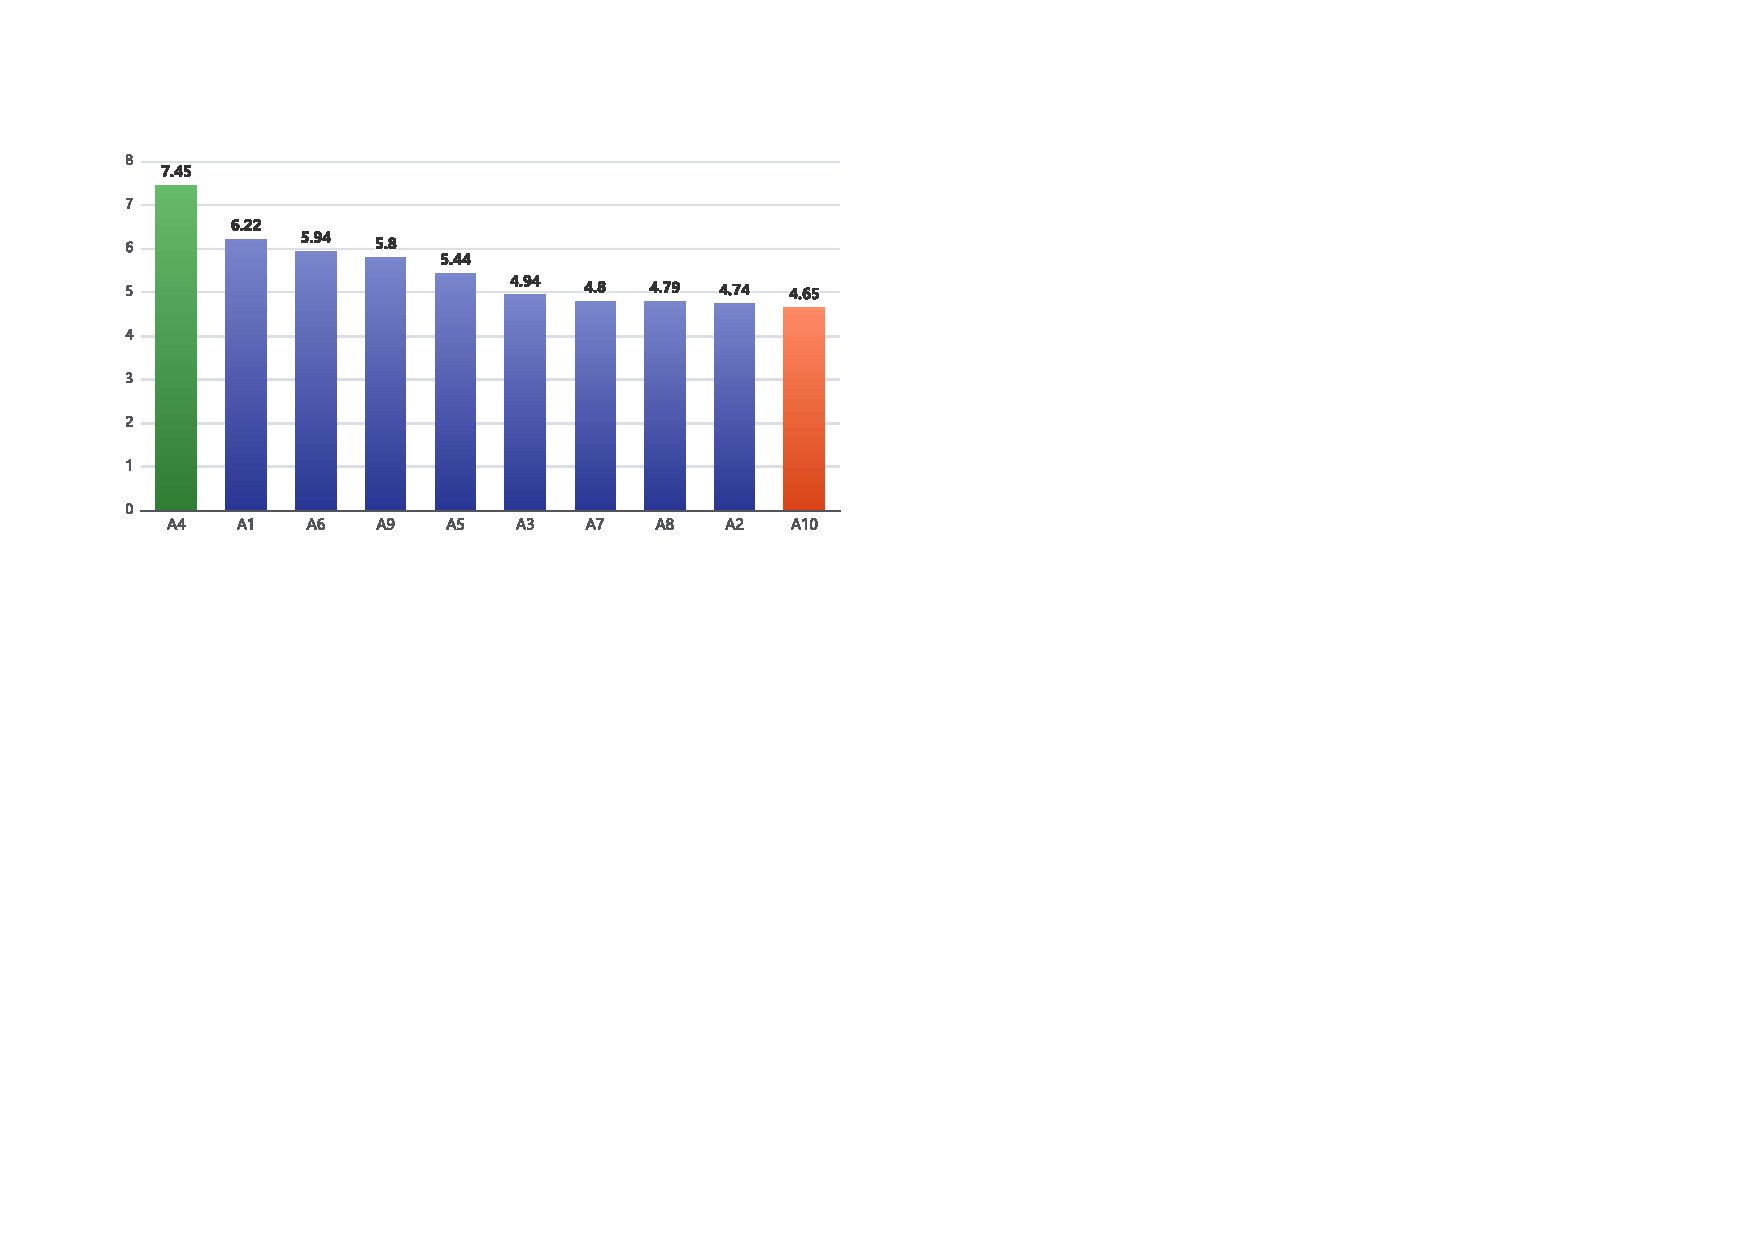
\includegraphics[
	width=.95\textwidth,
	trim=0cm 0cm 0cm 0cm, 
	clip
	]{figures/过滤器A1-A10寿命预测结果.pdf}
	\caption{过滤器A1-A10寿命预测结果}
	\label{fig:过滤器A1-A10寿命预测结果}
\end{figure}

各过滤器寿命从高到低排序为：A4、A1、A6、A9、A5、A3、A7、A8、A2、A10。A4过滤器耐久性最优，A10过滤器老化速度最快，需优先考虑更换计划。

\subsection{透水率预测特征分析}
选择过滤器A9展示预测结果并分析：

\begin{figure}[h!]
	\centering
	% trim = 左边裁剪 下边裁剪 右边裁剪 上边裁剪（单位：cm）
	% clip 表示启用裁剪功能
	\vspace{0cm}
	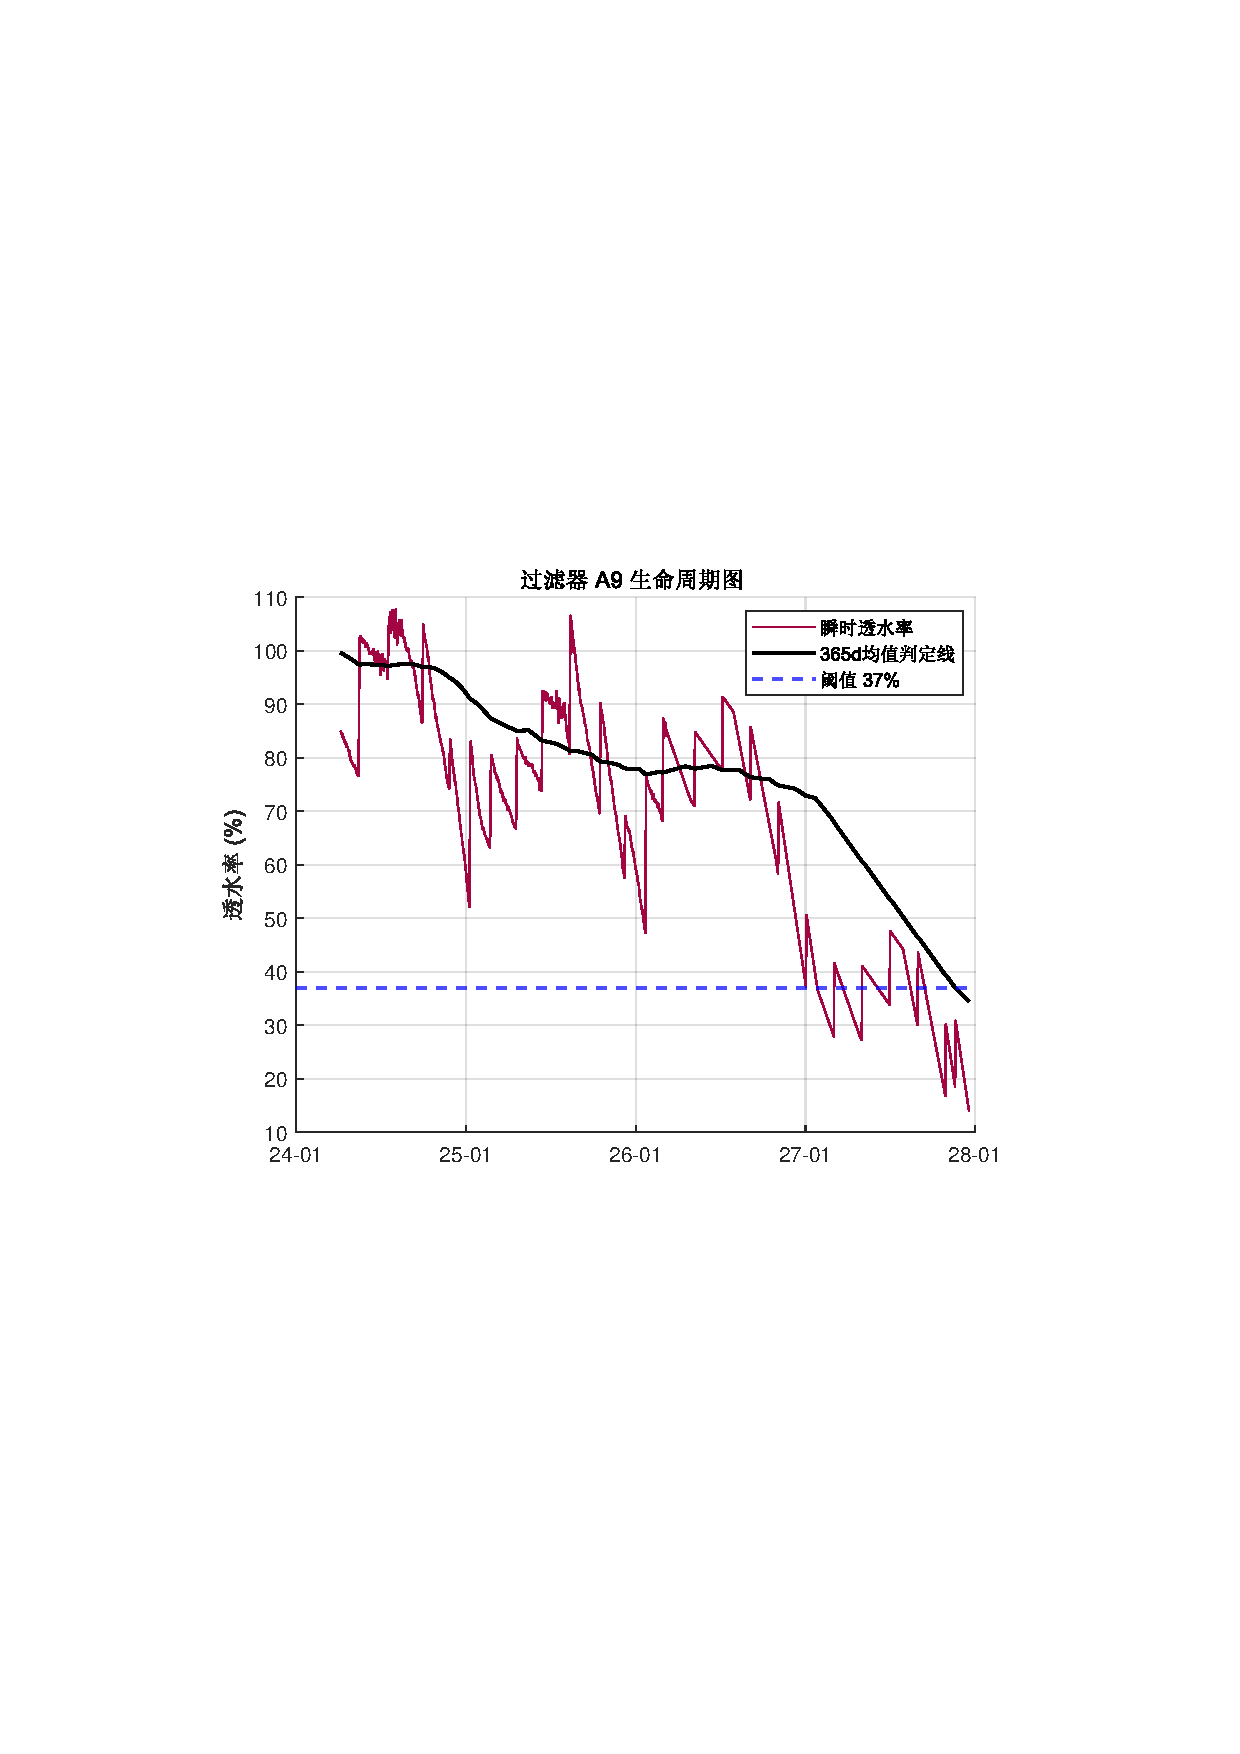
\includegraphics[
	width=.75\textwidth,
	trim=0cm 0cm 0cm 0cm, 
	clip
	]{figures/A9寿命预测.pdf}
	\caption{过滤器A9透水率预测曲线}
	\label{fig:A9寿命预测}
\end{figure}

由图~\ref{fig:A9寿命预测}，预测得到的瞬时透水率呈现典型的锯齿状演化形态，设备每60天执行一次中维护，使得透水率出现周期性瞬时回升，展现出显著的周期性波动与阶梯式衰减特征。随着设备服役时间延长与维护次数增加，内部损伤持续累积，中维护的性能恢复效果逐步衰减，透水率的回升幅度不断降低，整体劣化趋势持续加剧。

365天滑动平均曲线整体呈现平稳下降趋势，同时受季节影响呈现非线性变化特征：夏季劣化速率较慢，曲线走势平缓；秋冬季劣化速度加快，曲线下降趋势更为显著，符合第一问分析的结果。

当滑动平均线首次下穿37的寿命阈值时，模型自动触发紧急大维护进行性能补偿；若维护后30天内均值曲线仍无法恢复至阈值以上，或瞬时透水率接近失效临界值，则判定设备达到寿命终点。

\subsection{模型可靠性检验}
为了验证模型的预测可靠性，划分在附件中已知的透水率数据，把前70\%作为训练集用于模型参数辨识，后30\%作为测试集用于模型可靠性验证。将测试集预测的数据与原数据集进行对比，计算均方根误差RMSE与平均绝对百分比误差MAPE。
\begin{table}[H]
	\centering
	\setlength{\tabcolsep}{20pt}
	\renewcommand{\arraystretch}{1.5}
	\caption{各过滤器预测误差分析}
	\label{tab:模型可靠性}
	\begin{tabular}{ccc}
		\toprule
		\textbf{过滤器} & \textbf{MAPE (\%)} & \textbf{RMSE} \\
		\midrule
		\rowcolor{LightBlue}
		A1 & 22.109 & 21.43 \\
		A2 & 3.7066 & 2.4178 \\
		\rowcolor{LightBlue}
		A3 & 33.249 & 27.914 \\
		A4 & 7.0606 & 8.779 \\
		\rowcolor{LightBlue}
		A5 & 13.338 & 9.9052 \\
		A6 & 4.8007 & 5.4529 \\
		\rowcolor{LightBlue}
		A7 & 17.733 & 15.826 \\
		A8 & 6.331 & 5.4982 \\
		\rowcolor{LightBlue}
		A9 & 30.606 & 24.873 \\
		A10 & 9.8331 & 7.2135 \\
		\bottomrule
	\end{tabular}
\end{table}

由表~\ref{tab:模型可靠性}，在10台过滤器中，有7台过滤器的MAPE低于18\%，其中A2、A6、A8、A4、A10等5台过滤器的MAPE均低于10\%，A2和A6的MAPE分别仅为3.71\%和4.80\%，对应RMSE分别为2.42和5.45，预测精度优异。A3和A9的MAPE相对较高，分别为33.25\%和30.61\%，主要是由于该过滤器在验证期内经历了多次大维护，透水率波动剧烈，增加了预测难度。综上，模型对绝大多数过滤器具有可靠的预测能力。

现展示经过训练集参数确认后测试集与原数据集在2025年9月至2026年4月的可视化对比：

\newpage

\begin{figure}[h!]
	\centering
	% trim = 左边裁剪 下边裁剪 右边裁剪 上边裁剪（单位：cm）
	% clip 表示启用裁剪功能
	\vspace{0cm}
	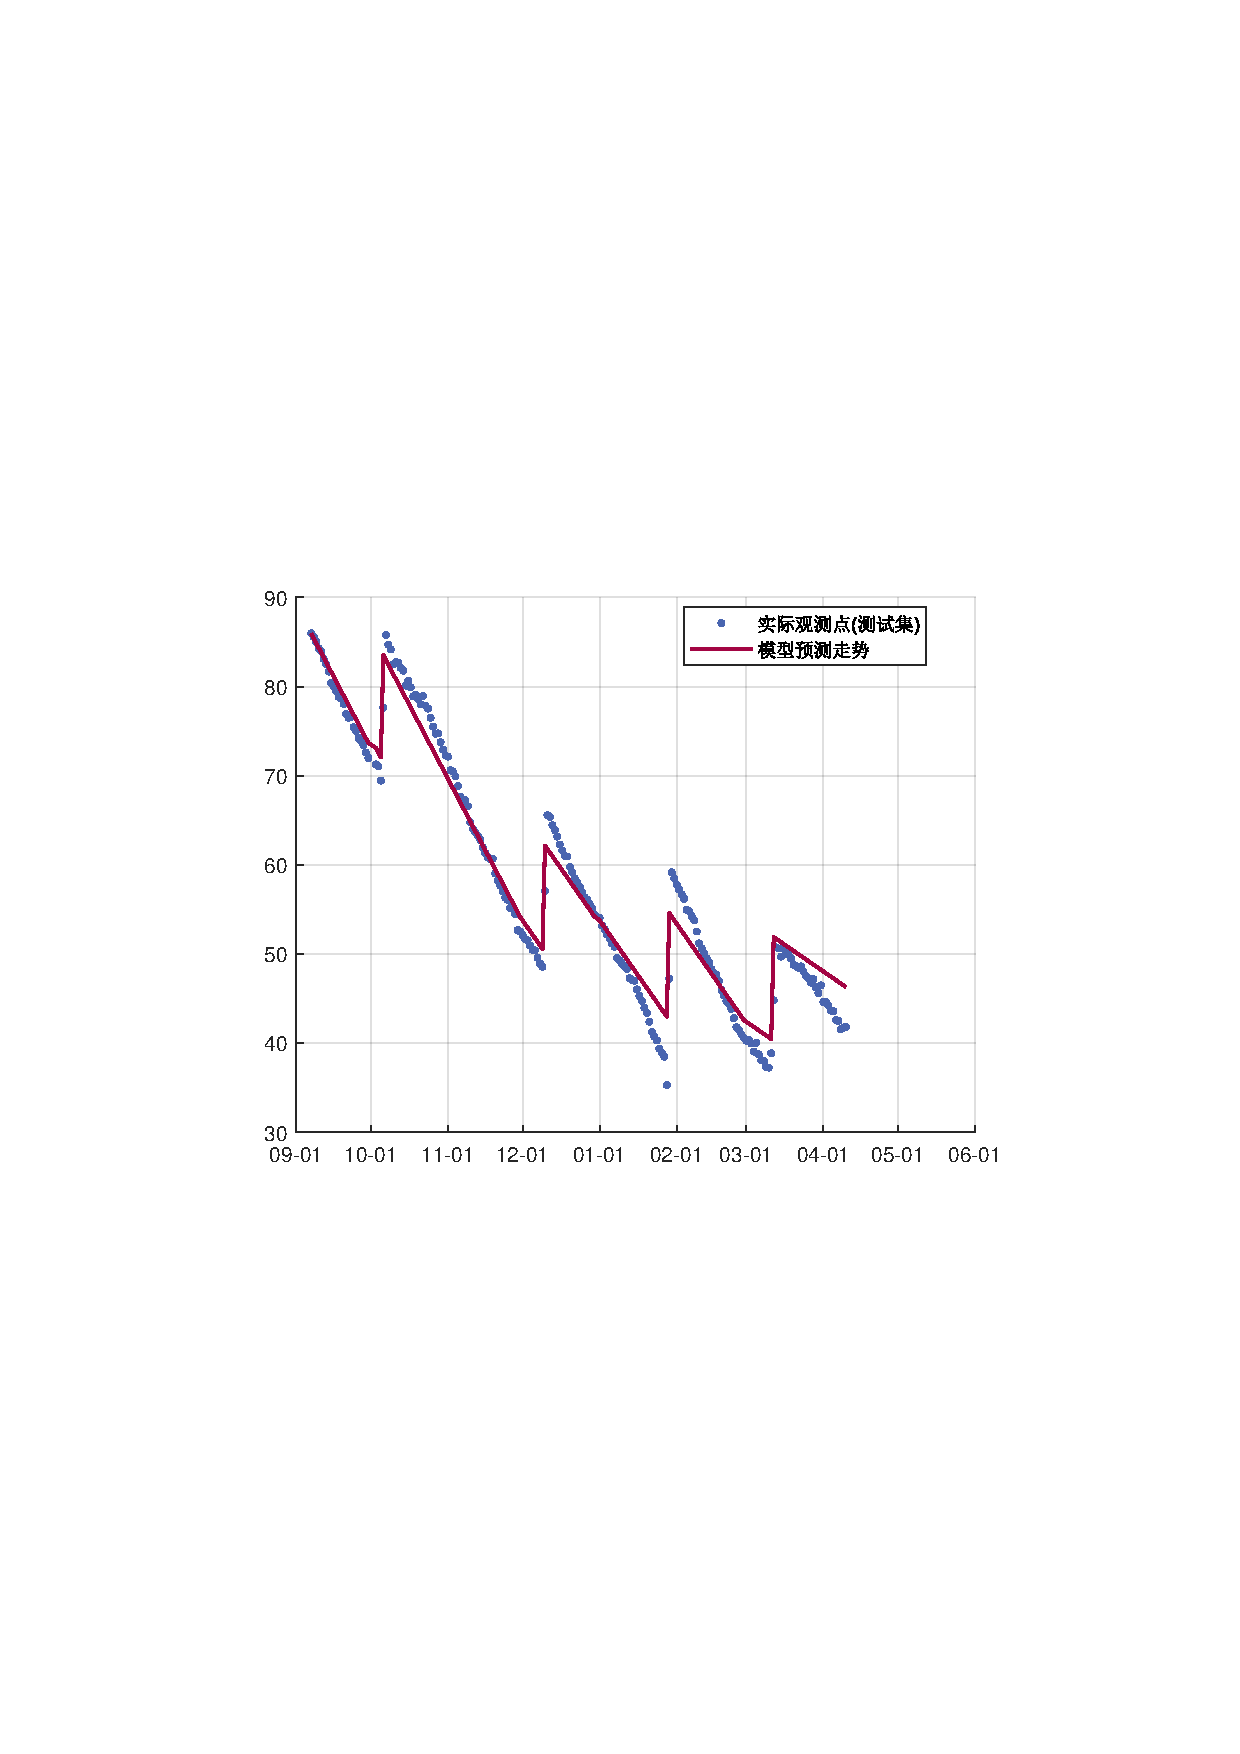
\includegraphics[
	width=.7\textwidth,
	trim=0cm 0cm 0cm 0cm, 
	clip
	]{figures/可靠性可视化.pdf}
	\caption{寿命预测模型预测值与实际值对比}
	\label{fig:可靠性可视化}
\end{figure}

由图 \ref {fig:可靠性可视化}，模型预测走势与原数据点的整体趋势一致、波动规律相同，表明模型的预测具备可靠性。




%%%%%%%%%%%%%%%%%%%%%%%%%%%%%%%%%%%%%%%%%%%%%%%%%%%%%%%%%%%%% 

\section{问题三的模型的建立和求解}

我们首先确定了计算过滤器一年成本的优化函数，根据现实情况确定决策变量，随即运用了前面两问建立的各项指标添加了约束条件，最后使用遗传算法求解，并对比了原来维护规律与我们建立的维护方案的年均成本。

\subsection{优化模型构建}

为了确定维护方案，在一个过滤器周期内的综合成本最小化，优化模型中优化函数、决策变量、约束条件制定如下。

\subsubsection{优化函数}

我们以一个过滤器从开始使用到寿命终止作为一个过滤器的生命周期，那么一个过滤器的生命周期的价格就是这个过滤器的价格再加上各种维护成本乘以维护次数，再用一个生命周期折算到一年的价格作为优化函数：
\begin{equation}
	\min \quad J(X) = \frac{C_{\text{purchase}} + c_{\text{mid}} \cdot n_{\text{mid}} + c_{\text{big}} \cdot n_{\text{big}}}{L},
\end{equation}
其中 $C_{\text{purchase}} = 300$ 万元为过滤器购买价格，$c_{\text{mid}} = 3$ 万元、$c_{\text{big}} = 12$ 万元分别为中维护与大维护的单次成本，$n_{\text{mid}}$、$n_{\text{big}}$ 为一个生命周期内两类维护的次数，$L$ 为过滤器寿命（年）。


\subsubsection{决策变量}

根据现实情况，当透水率下降较快时，或距离上次维护时间较长时，需要进行中维护；一年进行0-4次大维护。根据以上现实需要，我们制定了三个决策变量：
\begin{itemize}
	\item \textbf{中维护时间间隔阈值} $T_{\text{mid}}$：针对距离上次维护时间较长时需进行中维护的要求，设定当距离上次中维护的天数达到 $T_{\text{mid}}$ 时，进行一次中维护。
	\item \textbf{大维护时间间隔阈值} $T_{\text{big}}$：针对过滤器长期运行后性能严重衰减，需一年进行0-4次大维护的要求，设定当距离上次大维护的天数达到 $T_{\text{big}}$ 时，进行一次大维护。特别地，$T_{\text{big}}$可以大于一年的时间，于是一年可能没有大维护。
	\item \textbf{退化速率触发阈值} $r_{\text{th}}$：针对透水率下降速率较快时需进行中维护的要求，设定当近7天透水率的平均下降速率超过 $r_{\text{th}}$ 时，即使未达到固定间隔，也进行中维护。
\end{itemize}

于是决策向量由三个决策变量组合得到：
\begin{equation}
	X = (T_{\text{mid}},\ T_{\text{big}},\ r_{\text{th}}).
\end{equation}


\subsubsection{约束条件}

为确保优化结果符合工程实际，需对过滤器的运行状态、退化规律及维护触发逻辑施加约束，具体如下：

\begin{enumerate}[label=\bfseries\arabic*.]
	\item \textbf{确保过滤器始终处于可用状态}
	
	过滤器在任意时刻的透水率必须保持正值，否则意味着过滤器已完全失效，无法继续使用：
	\begin{equation}
		P(t) > 0, \quad \forall t.
	\end{equation}
	
	\item \textbf{确保长期平均透水率不低于37}
	
	只有365天滑动平均值低于37时才判定过滤器寿命终止，以消除短期波动干扰：
	\begin{equation}
		\bar{P}_{365}(t) = \frac{1}{365}\sum_{i=0}^{364} P(t-i), \quad \bar{P}_{365}(t) \geq 37,\ \forall t < L.
	\end{equation}
	
	\item \textbf{遵循第二问建立的状态转移演化规律}
	
	透水率的变化必须严格服从第二问所建立的状态转移方程，该方程综合了基准劣化、季节影响、维护损伤累积与维护增益的作用：
	\begin{equation}
		P(t+1) = P(t) - k_0 \cdot \beta_{s(t)} \cdot (1+\alpha_{\text{mid}})^{n_{\text{mid}}(t)} \cdot (1+\alpha_{\text{big}})^{n_{\text{big}}(t)} + G(t).
	\end{equation}
	
	\item \textbf{维护执行时机由决策变量控制}
	
	大维护按固定时间间隔 $T_{\text{big}}$ 执行，中维护在未触发大维护的前提下，由固定间隔 $T_{\text{mid}}$ 或下降速率过快两种方式触发：
	\begin{equation}
		\text{do}_{\text{big}} = \left( \Delta t_{\text{big}} \geq T_{\text{big}} \right),
	\end{equation}
	\begin{equation}
		\text{do}_{\text{mid}} = \neg \text{do}_{\text{big}} \land \left( \Delta t_{\text{mid}} \geq T_{\text{mid}} \lor \text{rate}(t) \leq -r_{\text{th}} \right),
	\end{equation}
	其中 $\text{rate}(t) = \dfrac{P(t) - P(t-7)}{7}$ 为过去7天的平均下降速率，$\Delta t_{\text{mid}}$、$\Delta t_{\text{big}}$ 分别为距上次中维护、大维护的时间间隔。
\end{enumerate}

综上，优化模型的完整约束条件为：
\[
	\left\{
	\begin{aligned}
		& P(t) > 0, \quad \forall t \\[4pt]
		& \bar{P}_{365}(t) = \frac{1}{365}\sum_{i=0}^{364} P(t-i), \quad \bar{P}_{365}(t) \geq 37,\ \forall t < L \\[4pt]
		& P(t+1) = P(t) - k_0 \cdot \beta_{s(t)} \cdot (1+\alpha_{\text{mid}})^{n_{\text{mid}}(t)} \cdot (1+\alpha_{\text{big}})^{n_{\text{big}}(t)} + G(t) \\[4pt]
		& \text{do}_{\text{big}} = \left( \Delta t_{\text{big}} \geq T_{\text{big}} \right) \\[4pt]
		& \text{do}_{\text{mid}} = \neg \text{do}_{\text{big}} \land \left( \Delta t_{\text{mid}} \geq T_{\text{mid}} \lor \text{rate}(t) \leq -r_{\text{th}} \right) \\[4pt]
		& \text{rate}(t) = \frac{P(t) - P(t-7)}{7}
	\end{aligned}
	\right.
\]

\subsection{利用遗传算法制定维护策略}

遗传算法是一类借鉴生物界自然选择和自然遗传机制的随机搜索算法。该算法模拟自然选择和自然遗传过程中发生的繁殖、交叉和基因突变现象，在每次迭代中保留一组候选解，并按适应度指标从解群中选取较优个体，利用遗传算子对这些个体进行组合产生新一代候选解群，重复此过程直至满足收敛指标\upcite{4}。与传统的启发式优化搜索算法相比，遗传算法的主要本质特征在于群体搜索策略和简单的遗传算子，群体搜索使算法能够突破领域搜索的限制，实现整个解空间上的分布式信息采集和探索；遗传算子仅利用适应值度量作为运算指标进行随机操作，降低了一般启发式算法在搜索过程中对人机交互的依赖。

基于该优化问题的以下三个特点，选择遗传算法求解：
\begin{itemize}
	\item \textbf{动态系统约束是非线性的}
	
	由状态转移方程 $P(t+1) = P(t) - k_0 \cdot \beta_{s(t)} \cdot (1+\alpha_{\text{mid}})^{n_{\text{mid}}(t)} \cdot (1+\alpha_{\text{big}})^{n_{\text{big}}(t)} + G(t)$ 可知，透水率每天的变化量不仅取决于当前值，还与维护次数 $n_{\text{mid}}$、$n_{\text{big}}$ 呈指数关系，那么维护次数越多，后续每天的劣化速度就越快。同时，季节因子 $\beta_{s(t)}$ 会在不同月时跳变，比如夏季约为0.4，秋季约为1.5，导致劣化速度相差近4倍。这些非线性、离散跳变和动态演化共同构成了复杂的约束体系。
	
	\item \textbf{维护行为会导致状态跳变}
	
	维护增益 $G(t)$ 的触发规则为 
	
	\vspace*{-10pt}
	\[\text{do}_{\text{mid}} = \neg \text{do}_{\text{big}} \land \left( \Delta t_{\text{mid}} \geq T_{\text{mid}} \lor \text{rate}(t) \leq -r_{\text{th}} \right),\]
	\vspace*{-20pt}
	
	当条件满足时，透水率会几乎突然增加， $G_{\text{mid}}$ 或 $G_{\text{big}}$会发生跳变，不是连续的。
	
	\item \textbf{目标函数不可解析表达}
	
	年均成本 $J = (300 + 3n_{\text{mid}} + 12n_{\text{big}}) / L$ 中的 $n_{\text{mid}}$、$n_{\text{big}}$ 和 $L$，无法写成关于 $T_{\text{mid}}$、$T_{\text{big}}$、$r_{\text{th}}$ 的公式。例如，$L$ 取决于逐日仿真中透水率何时跌破阈值、何时触发维护、衰减速率的累积效应等，这些过程包含大量条件判断和离散事件，无法用一个公式直接计算。
\end{itemize}

遗传算法不要求目标函数可导或可解析表达，仅需能够计算每个个体的适应度值，非常契合上述特点，因此采用遗传算法对该维护策略优化问题进行求解。

遗传算法参数设置如下：种群规模为30，最大进化代数为25，交叉概率0.7，变异概率0.05。决策变量搜索范围为：$T_{\text{mid}} \in [40, 120]$ 天，$T_{\text{big}} \in [150, 400]$ 天，$r_{\text{th}} \in [0.05, 1.5]$ 透水率/天。算法流程如下：

\vspace*{-15pt}
\[
	\begin{aligned}
		& \text{初始化种群 } \{X_1, X_2, \ldots, X_{N_{\text{pop}}}\} \\
		& \text{for } gen = 1 \text{ to } N_{\text{gen}}: \\
		& \quad \text{for each 个体 } X_i: \\
		& \quad \quad \text{运行寿命仿真，得 } L_i,\ n_{\text{mid}}^i,\ n_{\text{big}}^i \\
		& \quad \quad \text{计算适应度 } J_i = (300 + 3n_{\text{mid}}^i + 12n_{\text{big}}^i) / L_i \\
		& \quad \text{end} \\
		& \quad \text{选择、交叉、变异生成新一代种群} \\
		& \text{end} \\
		& \text{输出使 } J \text{ 最小的 } X^*
	\end{aligned}
\]

\vspace*{-5pt}
采用 MATLAB 内置遗传算法函数\texttt{ga}求解：
\begin{lstlisting}[language=Matlab, basicstyle=\small\ttfamily]
	bestX = ga(@(X) fitness_func(X, value_series, start_date, ...
	k0, S_vals, gm, gb, alpha_m, alpha_b, m_types, t_born), ...
	3, [], [], [], [], lb, ub, [], options);
\end{lstlisting}
其中 \texttt{fitness\_func} 为目标函数，返回给定决策变量 $X = (T_{\text{mid}}, T_{\text{big}}, r_{\text{th}})$ 下的年均成本；\texttt{lb}、\texttt{ub} 为决策变量下界与上界；\texttt{options} 通过 \texttt{optimoptions('ga', ...)} 设置种群规模为30、最大进化代数为25等参数。

\subsection{遗传算法的求解结果}

采用遗传算法对10台过滤器分别进行优化求解，得到的最优维护策略及对应寿命、年均成本如表~\ref{tab:遗传算法结果}所示：

\begin{table}[H]
	\centering
	\setlength{\tabcolsep}{6pt}
	\renewcommand{\arraystretch}{1.2}
	\caption{遗传算法优化结果}
	\label{tab:遗传算法结果}
	\begin{tabular}{lccccc}
		\toprule
		\textbf{过滤器} & \textbf{$L$（年）} & \textbf{$J$（万元）} & \textbf{$T_{\text{mid}}$（天）} & \textbf{$T_{\text{big}}$（天）} & \textbf{$r_{\text{th}}$} \\
		\midrule
		\rowcolor{LightBlue}
		A1 & 5.51 & 60.42 & 63 & 356 & 1.34 \\
		A2 & 4.53 & 66.87 & 115 & 273 & 1.33 \\
		\rowcolor{LightBlue}
		A3 & 4.68 & 64.80 & 120 & 277 & 1.20 \\
		A4 & 4.88 & 62.65 & 118 & 329 & 1.33 \\
		\rowcolor{LightBlue}
		A5 & 5.81 & 60.44 & 45 & 384 & 1.25 \\
		A6 & 5.72 & 59.24 & 62 & 379 & 1.15 \\
		\rowcolor{LightBlue}
		A7 & 4.60 & 65.88 & 114 & 399 & 1.15 \\
		A8 & 4.58 & 66.11 & 119 & 274 & 0.93 \\
		\rowcolor{LightBlue}
		A9 & 5.57 & 60.28 & 60 & 391 & 1.47 \\
		A10 & 4.55 & 66.59 & 115 & 310 & 1.14 \\
		\bottomrule
	\end{tabular}
\end{table}
其中 $L$ 为过滤器寿命（年），$J$ 为年均成本（万元/年），$T_{\text{mid}}$ 为中维护间隔阈值（天），$T_{\text{big}}$ 为大维护间隔阈值（天），$r_{\text{th}}$ 为退化速率触发阈值。经遗传算法优化后，工厂的污水净化年均成本，即10台过滤器的年均总成本为635.5万元。

为验证优化效果，将优化策略与第二问的原始固定维护策略进行对比，原始策略与优化策略的各过滤器的年均成本如表~\ref{tab:新旧对比}所示：

\begin{table}[H]
	\centering
	\setlength{\tabcolsep}{6pt}
	\renewcommand{\arraystretch}{1.2}
	\caption{优化策略与原始策略对比}
	\label{tab:新旧对比}
	\begin{tabular}{cccccc}
		\toprule
		\textbf{过滤器} & \textbf{优化后寿命} & \textbf{优化后年均成本} & \textbf{原始寿命} & \textbf{原始年均成本} & \textbf{成本波动} \\
		\midrule
		\rowcolor{LightBlue}
		A1 & 5.52 & 60.36 & 6.22 & 65.11 & -7.30\% \\
		A2 & 4.53 & 66.87 & 4.74 & 81.56 & -18.01\% \\
		\rowcolor{LightBlue}
		A3 & 4.72 & 64.87 & 4.94 & 75.32 & -13.88\% \\
		A4 & 4.88 & 62.65 & 7.45 & 53.56 & +16.97\% \\
		\rowcolor{LightBlue}
		A5 & 5.68 & 60.70 & 5.44 & 70.59 & -14.01\% \\
		A6 & 6.02 & 59.30 & 5.94 & 67.22 & -11.78\% \\
		\rowcolor{LightBlue}
		A7 & 4.60 & 65.88 & 4.80 & 76.84 & -14.26\% \\
		A8 & 4.58 & 66.11 & 4.79 & 73.34 & -9.85\% \\
		\rowcolor{LightBlue}
		A9 & 5.50 & 62.21 & 5.80 & 68.74 & -9.49\% \\
		A10 & 4.55 & 66.59 & 4.65 & 80.57 & -17.35\% \\
		\midrule
		\rowcolor{LightBlue}
		\textbf{平均} & \textbf{5.06} & \textbf{63.55} & \textbf{5.58} & \textbf{71.38} & \textbf{-11.04\%} \\
		\bottomrule
	\end{tabular}
\end{table}

由表~\ref{tab:新旧对比}，经遗传算法优化后，10台过滤器中有9台的年均成本较原始策略显著下降，平均降幅达11.04\%。其中A2、A10、A7、A5降幅最为明显，分别下降18.01\%、17.35\%、14.26\%和14.01\%，A3和A6降幅分别为13.88\%和11.78\%，验证了遗传算法在搜索最优维护策略方面的有效性。A8和A9降幅分别为9.85\%和9.49\%，A1降幅为7.30\%。A4过滤器成本上升16.97\%，主要由于其原始数据中缺乏大维护记录，导致参数辨识存在偏差，优化效果不显著。总体而言，优化策略在保证过滤器可靠运行的前提下，能够有效降低年均成本，验证了模型的有效性与实用性。

接下来选择过滤器A5在优化策略下的透水率预测曲线进行展示：

\begin{figure}[h!]
	\centering
	\vspace*{0pt}
	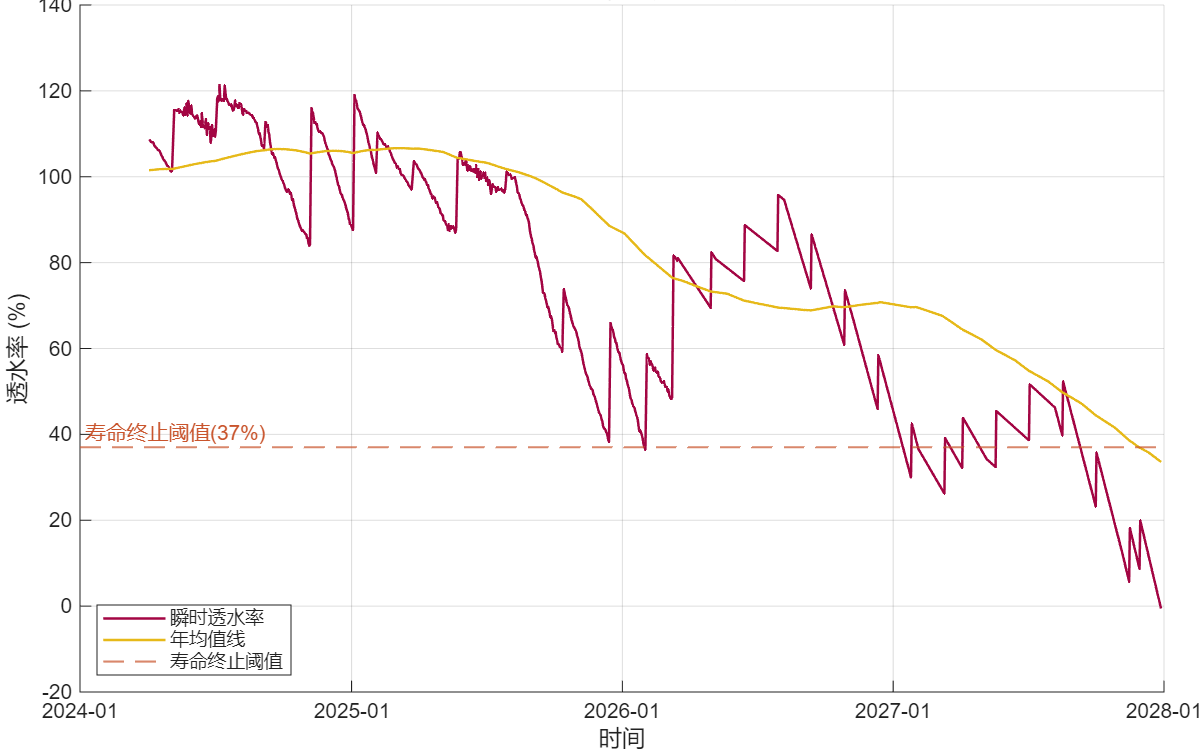
\includegraphics[width=0.8\textwidth,trim=0cm 0cm 0cm 0cm,clip]{figures/A5寿命预测.png}
	\caption{过滤器A5在新策略下的透水率预测曲线}
	\label{fig:A5新策略}
\end{figure}



%%%%%%%%%%%%%%%%%%%%%%%%%%%%%%%%%%%%%%%%%%%%%%%%%%%%%%%%%%%%% 

\vspace{-15pt}
\section{问题四的模型的建立和求解}

需要改变过滤器购买价格与维护成本来验证第三问的维护策略的稳健性，即对过滤器购买价格与维护成本进行敏感性分析。在题目给的三个价格参数的基础上，设置四类波动情景：购买价格单独波动、维护成本单独波动、全部成本同向波动、购买价格与维护成本反向波动，波动幅度为 $\pm 10\%$ 和 $\pm 15\%$。

为了衡量第三问建立的策略在新成本下的表现，设损失率 $\delta$ 为：
\begin{equation}
	\delta = \frac{A_{\text{fixed}} - A_{\text{opt}}}{A_{\text{opt}}} \times 100\%,
\end{equation}
其中， $A_{\text{fixed}}$ 为保持原维护策略不变、仅替换成本单价后计算得到的年均成本；$A_{\text{opt}}$ 为在新成本参数下重新优化得到的最优年均成本。$\delta$ 为正表示原策略优于重新优化策略，为负表示原策略劣于重新优化策略。$|\delta| \leq 3\%$ 代表原方案完全可行，$3\% < |\delta| \leq 5\%$ 代表模型轻微敏感。

选择展示过滤器 A1 在所有参数波动情景下的敏感性分析结果：

\begin{table}[H]
	\centering
	\setlength{\tabcolsep}{4pt}
	\renewcommand{\arraystretch}{1.2}
	\caption{过滤器 A1 成本敏感性分析结果}
	\label{tab:A1灵敏度分析}
	\begin{tabular}{lccc}
		\toprule
		\textbf{情景} & \textbf{$A_{\text{fixed}}$（万元）} & \textbf{$A_{\text{opt}}$（万元）} & \textbf{$\delta$（\%）} \\
		\midrule
		\rowcolor{LightBlue}
		购买价格 +10\% & 65.86 & 65.80 & 0.10 \\
		购买价格 -10\% & 54.98 & 55.03 & -0.09 \\
		\rowcolor{LightBlue}
		购买价格 +15\% & 68.59 & 69.00 & -0.60 \\
		购买价格 -15\% & 52.26 & 52.20 & 0.10 \\
		\midrule
		\rowcolor{LightBlue}
		维护成本 +10\% & 61.02 & 60.99 & 0.05 \\
		维护成本 -10\% & 59.82 & 60.15 & -0.55 \\
		\rowcolor{LightBlue}
		维护成本 +15\% & 61.32 & 61.27 & 0.08 \\
		维护成本 -15\% & 59.52 & 59.49 & 0.05 \\
		\midrule
		\rowcolor{LightBlue}
		全部成本 +10\% & 66.46 & 66.63 & -0.24 \\
		全部成本 -10\% & 54.38 & 54.38 & 0.00 \\
		\rowcolor{LightBlue}
		全部成本 +15\% & 69.48 & 71.89 & -3.34 \\
		全部成本 -15\% & 51.36 & 51.34 & 0.04 \\
		\midrule
		\rowcolor{LightBlue}
		购买价格+10\% 维护成本-10\% & 65.27 & 66.11 & -1.28 \\
		购买价格-10\% 维护成本+10\% & 55.58 & 55.72 & -0.25 \\
		\rowcolor{LightBlue}
		购买价格+15\% 维护成本-15\% & 67.69 & 67.65 & 0.06 \\
		购买价格-15\% 维护成本+15\% & 53.15 & 53.15 & 0.00 \\
		\bottomrule
	\end{tabular}
\end{table}

由表~\ref{tab:A1灵敏度分析}，在所有测试情景下，损失率 $\delta$ 的绝对值均不超过 3.34\%，其中绝大多数情景的 $|\delta|$ 小于 2\%。仅当全部成本上涨 15\% 时，$\delta = -3.34\%$，略超过 3\% 阈值，但仍处于可接受范围内。综上，第三问的最优维护策略在购买价格和维护成本发生 $\pm 15\%$ 以内的变化时体现出良好的稳健性。

\begin{figure}[h!]
	\centering
	\vspace*{0pt}
	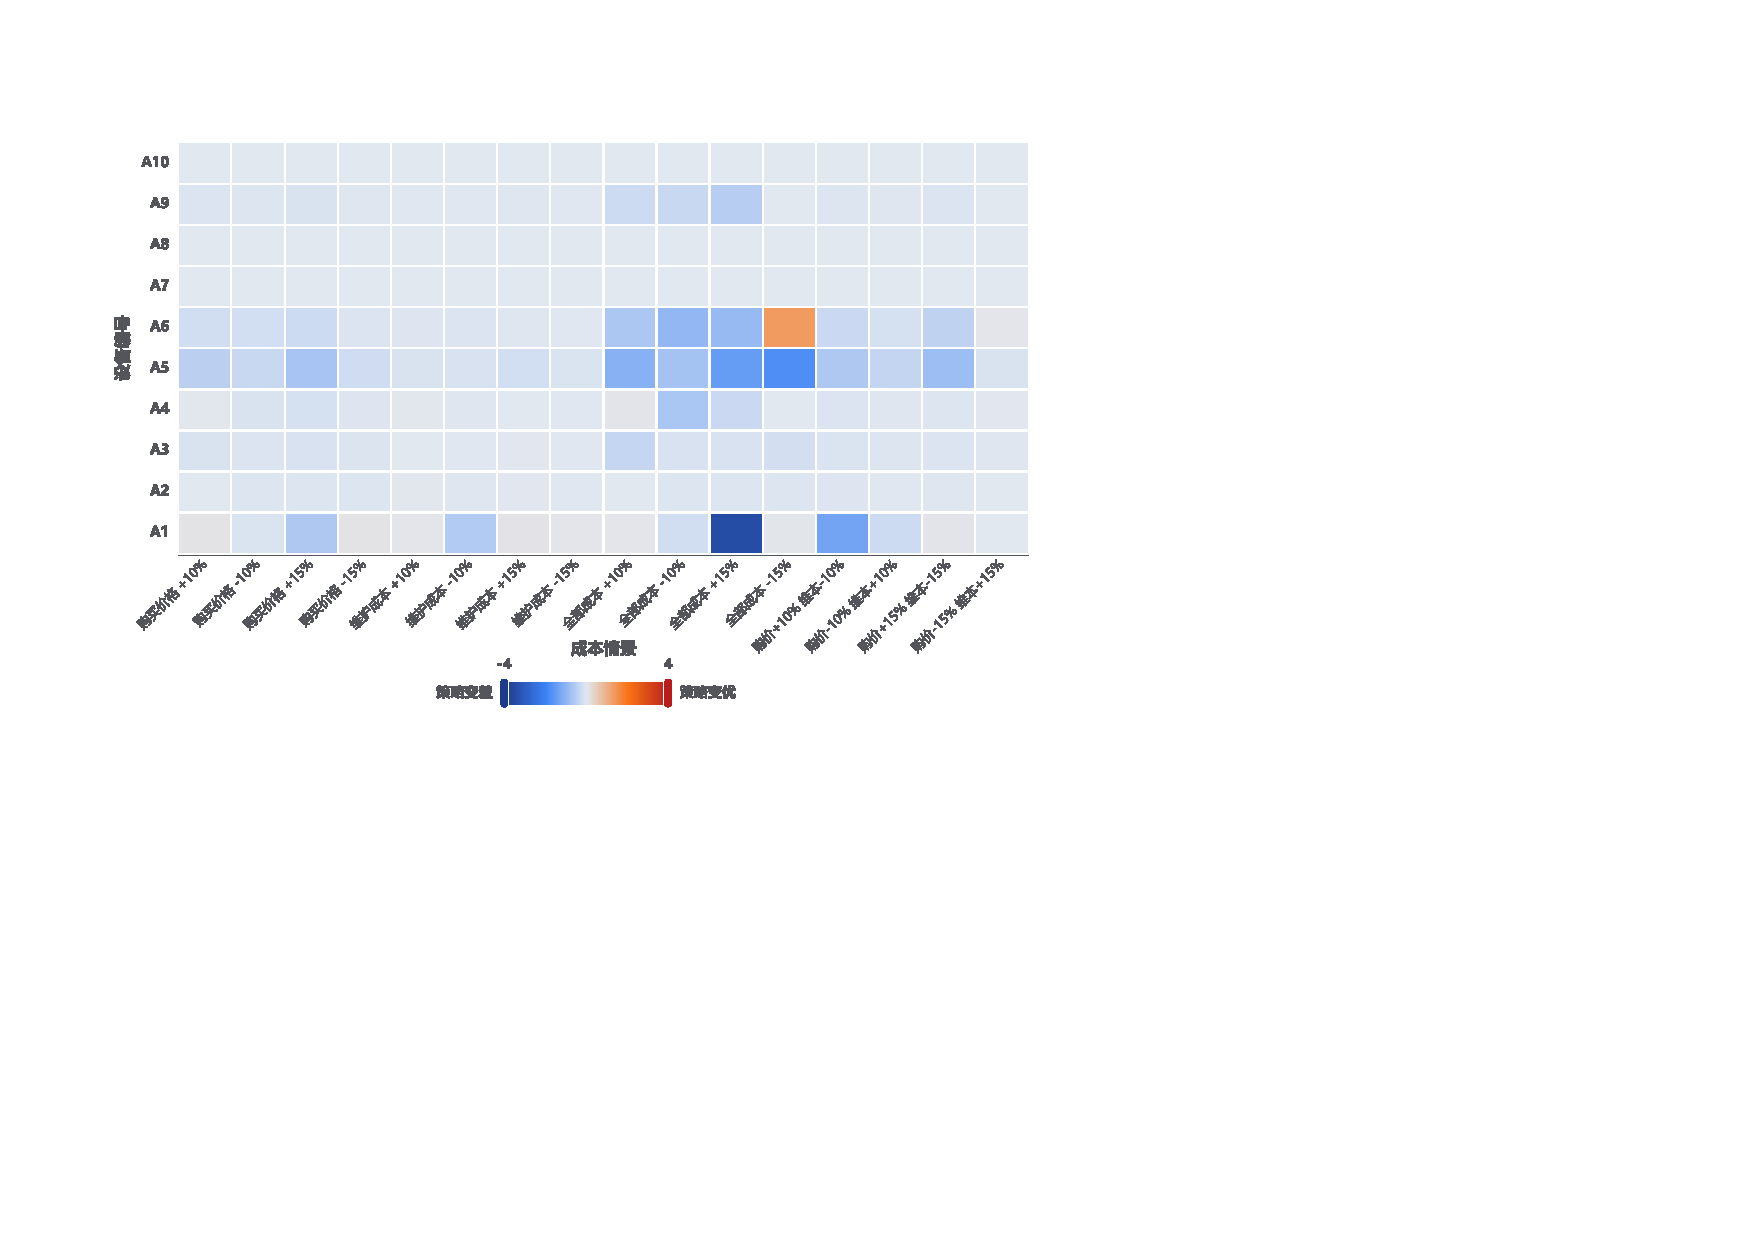
\includegraphics[width=0.85\textwidth,trim=0cm 0cm 0cm 0.3cm,clip]{figures/损失率热力图.pdf}
	\caption{过滤器维护策略损失率热力图}
	\label{fig:损失率热力图}
\end{figure}

由图~\ref{fig:损失率热力图}，绝大多数 $\delta$ 值落在 $-1\%$ 至 $1\%$ 之间，A7、A8、A10 在所有情景下 $\delta$ 均为零，A5 和 A6 的 $\delta$ 绝对值略高但不超过 $1.70\%$，所有情景最大的 $|\delta|$ 为 A1 在全部成本上涨 $15\%$ 时的 $-3.34\%$。所有 $|\delta|$ 均控制在 $3.34\%$ 以内，验证了最优维护策略在成本波动下的良好稳健性。

对所有设备在全部成本波动情景下的损失率进行展示：

\begin{table}[H]
	\centering
	\setlength{\tabcolsep}{4pt}
	\renewcommand{\arraystretch}{1.2}
	\caption{全部过滤器在全部成本波动下的损失率（\%）}
	\label{tab:所有灵敏度分析}
	\begin{tabular}{ccccc}
		\toprule
		\textbf{过滤器} & \textbf{全部成本 +10\%} & \textbf{全部成本 -10\%} & \textbf{全部成本 +15\%} & \textbf{全部成本 -15\%} \\
		\midrule
		\rowcolor{LightBlue}
		A1 & 0.05 & -0.20 & 0.11 & 0.06 \\
		A2 & 0.00 & -0.06 & -0.06 & -0.06 \\
		\rowcolor{LightBlue}
		A3 & -0.34 & -0.11 & -0.11 & -0.17 \\
		A4 & 0.06 & -0.64 & -0.28 & 0.00 \\
		\rowcolor{LightBlue}
		A5 & -1.03 & -0.71 & -1.44 & -1.70 \\
		A6 & -0.62 & -0.92 & -0.86 & 1.26 \\
		\rowcolor{LightBlue}
		A7 & 0.00 & 0.00 & 0.00 & 0.00 \\
		A8 & 0.00 & 0.00 & 0.00 & 0.00 \\
		\rowcolor{LightBlue}
		A9 & -0.25 & -0.30 & -0.49 & 0.00 \\
		A10 & 0.00 & 0.00 & 0.00 & 0.00 \\
		\bottomrule
	\end{tabular}
\end{table}
由表~\ref{tab:所有灵敏度分析}，在全部成本同向波动 $\pm 10\%$ 和 $\pm 15\%$ 的情景下，所有过滤器的损失率绝对值均未超过 1.70\%，远低于 3\% 的可行性阈值。其中 A7、A8、A10 三台设备的损失率在所有情景下均为 0，表明其原最优策略在成本波动后依然处于最优解附近。A2 的损失率绝对值最大为 0.06\%，A1 和 A4 的损失率绝对值均在 0.64\% 以内，A3 和 A9 的损失率绝对值均在 0.49\% 以内，均表现稳定。A5 和 A6 的损失率相对略高，A5 在全部成本下降 15\% 时损失率为 -1.70\%，A6 在同一情景下损失率为 1.26\%，但绝对值仍远低于 3\% 的阈值。综合全部设备的分析结果，第三问所求得的最优维护策略在成本发生 $\pm 10\% \sim \pm 15\%$ 波动时具有良好的普适性和稳健性，无需因市场价格波动而调整维护方案。

%%%%%%%%%%%%%%%%%%%%%%%%%%%%%%%%%%%%%%%%%%%%%%%%%%%%%%%%%%%%%

%\section{模型的分析与检验}

%\subsection{灵敏度分析}

%\subsection{误差分析}

%%%%%%%%%%%%%%%%%%%%%%%%%%%%%%%%%%%%%%%%%%%%%%%%%%%%%%%%%%%%%

\section{模型的评价}

\subsection{模型的优点}

\begin{itemize}
	\item \textbf{数据预处理充分}：采用改进的自适应 Hampel 滤波器对原始数据进行清洗，有效剔除了异常波动并保留维护引发的真实阶跃信号。
	
	\item \textbf{物理意义清晰}：模型综合考虑了具有明确物理含义的自然衰减、季节影响、维护增益与损伤四项指标，避免了单一因素分析的片面性与黑箱模型的不可解释性。
	
	\item \textbf{模型可解释性强}：透水率状态转移方程基于实际物理过程构建，各参数均可从数据中辨识，避免了黑箱模型难以解释的弊端。
	
	\item \textbf{优化方法适用性强}：以年均成本最小化为目标函数，将维护间隔与速率阈值作为决策变量，采用遗传算法全局寻优，有效处理了离散决策变量与非线性目标函数的组合优化问题，对各设备均能稳定获得合理方案，复现性良好。
	
	\item \textbf{模型泛化性良好}：模型可推广应用于不同型号、不同工况的过滤设备。只需根据具体设备的透水率监测数据重新辨识衰减系数、季节算子、损伤系数等核心参数，即可适配不同设备的性能特征与维护需求，具有较强的可扩展性。
\end{itemize}

\subsection{模型的缺点}

\begin{itemize}
	\item \textbf{未考虑小维护的影响}：由于小维护成本可忽略且单次效果微弱，没有将其纳入模型。对于小维护效果显著的场景，模型可能需要进一步扩展。
	
	\item \textbf{季节影响采用离散跳变}：季节算子按月离散取值，未能刻画季节交替过程中的连续过渡特征，可能引入一定近似误差。
\end{itemize}

\subsection{模型的改进方向}

\begin{itemize}
	\item \textbf{精细化季节影响建模}：当前季节算子按月离散跳变，未来可采用连续函数拟合季节波动，更精确地刻画季节交替过程中的过渡特征。
	
	\item \textbf{引入参数不确定性量化}：透水率检测存在测量噪声，参数辨识和寿命预测结果存在不确定性，未来可引入贝叶斯方法等概率模型对不确定性进行量化。
	
	\item \textbf{考虑外部环境的随机波动}：后续可引入随机微分方程或蒙特卡洛仿真，进一步描述污水水质、操作条件、气候条件变化等随机波动对模型的影响，提升对不确定因素的量化能力与决策的稳健性。
	
\end{itemize}

\subsection{模型的推广}

\begin{itemize}
	\item \textbf{适用其他工业设备的维护优化}：模型可推广至其他存在性能退化且需要定期维护的工业设备，如空气过滤器、油液过滤器、膜分离设备等。
	
	\item \textbf{可包容更多影响因素}：模型框架可扩展纳入更多影响因素，如操作压力、流量、温度等实时运行参数，只需要将参数纳入状态转移方程即可。
	
	\item \textbf{可扩展至多目标优化方案}：当前以年均成本最小为单目标，同时也具有可扩展为多目标优化，只需要添加对应参数至优化函数，并添加对应决策变量及限制条件即可。
\end{itemize}

%%%%%%%%%%%%%%%%%%%%%%%%%%%%%%%%%%%%%%%%%%%%%%%%%%%%%%%%%%%%%
%% 参考文献

\newpage

\nocite{*}
\begin{thebibliography}{9}%宽度9
\bibitem{1} 谢宇轩,范琳琳,郭鑫,等.基于Hampel滤波的海洋磁测数据异常值检测方法研究[J].海洋学报,2025,47(04):53-64.
\bibitem{2} 张闻胜,王银堂.时间序列分解模型在水文要素中长期预报中的应用[J].水文,2001,(01):21-24.
\bibitem{3} CJJ 60-2011, 城镇污水处理厂运行、维护及安全技术规程 [S]. 北京：中国建筑工业出版社，2011.
\bibitem{4} 边霞,米良.遗传算法理论及其应用研究进展[J].计算机应用研究,2010,27(07):2425-2429+2434.
\end{thebibliography}
%%%%%%%%%%%%%%%%%%%%%%%%%%%%%%%%%%%%%%%%%%%%%%%%%%%%%%%%%%%%%
%% 附录
\begin{appendices}
\section{支撑材料的文件列表}
\begin{table}[H]
	\centering
	\setlength{\tabcolsep}{6pt}
	\renewcommand{\arraystretch}{1.5}
	%\caption{支撑材料文件列表}
	\label{tab:支撑材料}
	\begin{tabular}{lc}
		\toprule
		\textbf{文件名} & \textbf{功能描述} \\
		\midrule
		\rowcolor{LightBlue}
		附件1整合数据.xlsx & 用于读入代码的数据表 \\
		附件2整合数据.xlsx & 用于读入代码的数据表 \\
		\rowcolor{LightBlue}
		Q1\_Hampel\_All.m & 第一问进行异常值处理的代码 \\
		Q1\_STL.m & 第一问进行时间序列分解的代码 \\
		\rowcolor{LightBlue}
		Q1\_Parameter.m & 第一问下降趋势规律分析代码 \\
		Q2\_Finalist.m & 第二问参数确定与寿命预测代码 \\
		\rowcolor{LightBlue}
		Q2\_Reliability.m & 第二问模型可靠性检验代码 \\
		Q3Q4.m & 第三、四问利用遗传算法进行优化模型求解以及参数扰动检验代码 \\
		\bottomrule
	\end{tabular}
\end{table}

\section{代码}
\noindent Q1\_Hampel\_All.m
\lstinputlisting[language=matlab]{code/Q1_Hampel_All.m}

\noindent Q1\_STL.m
\lstinputlisting[language=matlab]{code/Q1_STL.m}

\noindent Q1\_Parameter.m
\lstinputlisting[language=matlab]{code/Q1_Parameter.m}

\noindent Q2\_Finalist.m
\lstinputlisting[language=matlab]{code/Q2_Finalist.m}

\noindent Q2\_Reliability.m
\lstinputlisting[language=matlab]{code/Q2_Reliability.m}

\noindent Q3Q4.m
\lstinputlisting[language=matlab]{code/Q3Q4.m}
\end{appendices}
\end{document}


